\documentclass[sigconf]{acmart}

\AtBeginDocument{%
  \providecommand\BibTeX{{%
    Bib\TeX}}}

\setcopyright{none}

\usepackage{booktabs}
\usepackage{graphicx}
\usepackage{subcaption}
\usepackage[section]{placeins}
\usepackage{url}
\usepackage{tikz}
\usetikzlibrary{arrows.meta, positioning, shapes.geometric}
\usepackage{multirow}
\usepackage{xcolor}

\renewcommand\footnotetextcopyrightpermission[1]{}

\acmConference{}{}{}
\acmBooktitle{}
\acmPrice{}
\acmDOI{}
\acmISBN{}
\settopmatter{printacmref=false}

\begin{document}

\title{Mouse Well-Being Classification from Muzzle Images}

\author{Qingyun Chen}
\author{Burak Hafizoglu}
\affiliation{%
  \institution{Technische Universit\"at Berlin}
  \city{Berlin}
  \country{Germany}
}

\begin{abstract}
Assessing the well-being of laboratory mice is essential for animal welfare
and biomedical research. Manual Mouse Grimace Scale (MGS) scoring is reliable
but labor-intensive and subject to observer variability. Motivated by evidence
that facial appearance---and particularly the muzzle---carries welfare-related
cues, we study whether binary well-being status
(\textit{impaired} vs.\ \textit{not impaired}) can be predicted from images
using convolutional neural networks. We construct labels from multi-rater MGS
facial-action-unit scores, compare muzzle crops against matched full-face
images, and evaluate ResNet18 and ConvNeXt-Tiny under controlled ablations of
augmentation and fine-tuning choices. On a held-out test set, the best overall
model is a full-image ResNet18 with light augmentation and learning rate
$5\times10^{-5}$ (Macro-F1 $=0.838$). The best crop-only model is ConvNeXt-Tiny
with light augmentation and dropout $0.0$ (Macro-F1 $=0.812$). The results
support the feasibility of automatic muzzle-based well-being classification
and provide a reproducible ablation baseline for non-invasive monitoring.
\end{abstract}

\maketitle

%% ================================================================
%%  INTRODUCTION
%% ================================================================
\section{Introduction}
Laboratory mice play a central role in biomedical research, making reliable
assessment of their well-being essential for both animal welfare and
scientific practice. Ethical frameworks such as the 3Rs---replace, reduce, and
refine---encourage methods that improve welfare monitoring while reducing
burden on animals and experimenters. The Mouse Grimace Scale (MGS) provides a
standardized approach to assess pain and discomfort from facial action units
\cite{Langford2010}. However, manual scoring requires trained experts, is
time-consuming, and can introduce observer variability, limiting large-scale
application.

Computer vision offers a path toward objective and scalable assessment.
Markerless pose estimation with DeepLabCut showed that deep networks can
localize animal landmarks from limited labels \cite{Mathis2018}. Subsequent
work automated aspects of MGS scoring under varied recording conditions
\cite{Andresen2026}, and Reimann et al.\ reported that modern vision models
align with human MGS assessment while suggesting that cues beyond classical
action units---including muzzle appearance---contribute to performance
\cite{Reimann2026}. These findings raise a concrete question:

\begin{quote}
\textit{Can mouse well-being be classified accurately from images, and how much
information is retained when using muzzle crops alone?}
\end{quote}

In this work, we address that question with a controlled ablation study.
We build binary labels from available MGS scores, prepare paired muzzle-crop
and full-image inputs for the same samples, and fine-tune ImageNet-pretrained
ResNet18 \cite{He2016} and ConvNeXt-Tiny \cite{Liu2022}. Part~1 varies
architecture, input type, and augmentation. Part~2 tunes learning rate,
dropout, and backbone freezing on the strongest Part~1 settings. Our contributions are:
\begin{enumerate}
  \item a reproducible binary classification pipeline for mouse well-being
  from MGS-derived labels;
  \item a systematic comparison of muzzle crops versus full images under
  identical splits and identities;
  \item ablation evidence that light augmentation and careful fine-tuning
  improve Macro-F1, while freezing the backbone hurts.
\end{enumerate}

%% ================================================================
%%  RELATED WORK
%% ================================================================
\section{Related Work}

The Mouse Grimace Scale, introduced by Langford et al.~\cite{Langford2010},
scores facial action units such as orbital tightening, nose bulge, cheek
bulge, ear position, and whisker change on a $0/1/2$ scale. Although MGS is
widely used, it depends on human raters.

DeepLabCut demonstrated that transfer learning with convolutional networks
enables accurate markerless pose estimation for user-defined animal body parts
\cite{Mathis2018}. Building on related advances, Andresen et al.~\cite{Andresen2026}
studied automatic pain-face analysis in mice under non-standardized
conditions. Dolensek et al.~\cite{Dolensek2020} showed that mice express
emotion-specific facial configurations with corresponding neural correlates,
indicating that facial appearance encodes rich internal state information.

Most directly related, Reimann et al.~\cite{Reimann2026} compared computer-vision
paradigms with human MGS assessment and reported indications that muzzle shape
reflects well-being. Our work follows this motivation but focuses on a
practical binary task and a transparent ablation of input type (crop vs.\ full),
architecture (ResNet18 vs.\ ConvNeXt-Tiny), and training choices.

%% ================================================================
%%  METHOD
%% ================================================================
\section{Method}
\label{sec:method}

Our framework consists of five stages: label construction, image preparation,
dataset splitting, model training, and test-set evaluation.
Figure~\ref{fig:pipeline} summarizes the pipeline used throughout the
experiments.

\begin{figure}[t]
  \centering
  \resizebox{\linewidth}{!}{%
  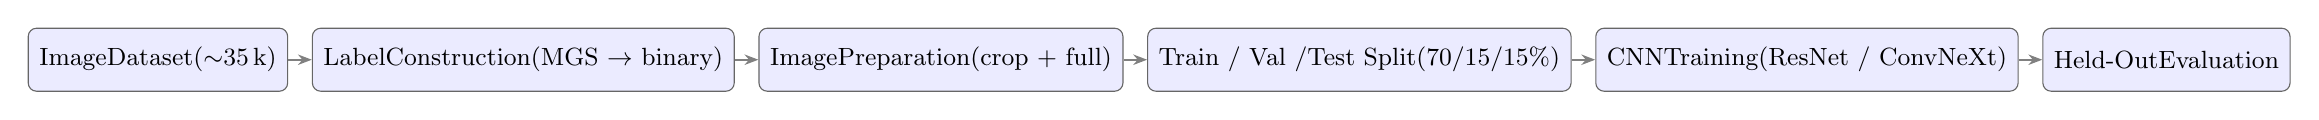
\begin{tikzpicture}[
    node distance=0.5cm and 0.3cm,
    block/.style={
      rectangle, rounded corners=3pt,
      draw=black!60, fill=blue!8,
      minimum height=0.8cm, minimum width=2.0cm,
      text centered, font=\small,
      inner sep=4pt
    },
    arrow/.style={-{Stealth[length=5pt]}, thick, draw=black!50}
  ]
    \node[block] (data) {Image\\Dataset\\($\sim$35\,k)};
    \node[block, right=of data] (label) {Label\\Construction\\(MGS $\to$ binary)};
    \node[block, right=of label] (prep) {Image\\Preparation\\(crop + full)};
    \node[block, right=of prep] (split) {Train / Val /\\Test Split\\(70/15/15\%)};
    \node[block, right=of split] (train) {CNN\\Training\\(ResNet / ConvNeXt)};
    \node[block, right=of train] (eval) {Held-Out\\Evaluation};

    \draw[arrow] (data) -- (label);
    \draw[arrow] (label) -- (prep);
    \draw[arrow] (prep) -- (split);
    \draw[arrow] (split) -- (train);
    \draw[arrow] (train) -- (eval);
  \end{tikzpicture}}
  \caption{Overview of the classification pipeline. Images are resized to
  $224\times224$, normalized with ImageNet statistics, and classified with
  ImageNet-pretrained CNNs. Early stopping monitors validation Macro-F1; the
  test threshold is fixed at $0.5$.}
  \label{fig:pipeline}
\end{figure}

\subsection{Dataset and Label Construction}
\label{subsec:label-construction}

The original collection contained on the order of $35{,}000$ mouse images from
five subsets (AW, JW, KH, LW, MR). MGS annotations were available for only a
fraction of images and included multiple expert ratings for nose bulge (nb),
cheek bulge (cb), and whisker change (wc).

Invalid and missing annotations were removed: empty entries, ``-'', and the
invalid score value $9$ were ignored. Let $\mathcal{S}_i$ denote the set of
all valid facial-action-unit scores for image $i$. The pooled mean score is
\begin{equation}
    m_i =
    \frac{1}{|\mathcal{S}_i|}
    \sum_{s \in \mathcal{S}_i} s.
\end{equation}
Images without any valid score were excluded. Binary labels were obtained by
\begin{equation}
    y_i =
    \begin{cases}
        1, & m_i \geq 0.5,\\
        0, & m_i < 0.5,
    \end{cases}
\end{equation}
where $y_i=1$ denotes \textit{impaired} and $y_i=0$ denotes \textit{not
impaired}. After filtering and class balancing for the curated experimental
set used in this study, the working dataset contained $1{,}778$ images with
equal class counts ($889$ per class).

Table~\ref{tab:dataset} shows the distribution of images across subsets and
splits. The five subsets originate from different experimental cohorts,
introducing natural variation in lighting, camera angle, and mouse strain.
Subset sizes range from $n=26$ (AW) to $n=574$ (MR), creating an
imbalanced contribution to training and evaluation.

\begin{table}[t]
  \centering
  \caption{Dataset distribution across subsets and splits. Each cell shows the
  number of images (not-impaired / impaired).}
  \label{tab:dataset}
  \small
  \begin{tabular}{lccc|c}
    \toprule
    Subset & Train & Val & Test & Total \\
    \midrule
    AW & 62\,(37/25)  & 13\,(8/5)   & 13\,(8/5)   & 88  \\
    JW & 262\,(105/157) & 56\,(23/33) & 56\,(23/33) & 374 \\
    KH & 362\,(156/206) & 77\,(33/44) & 77\,(33/44) & 516 \\
    LW & 158\,(133/25)  & 34\,(29/5)  & 34\,(29/5)  & 226 \\
    MR & 402\,(190/212) & 86\,(41/45) & 86\,(41/45) & 574 \\
    \midrule
    Total & 1{,}246 & 266 & 266 & 1{,}778 \\
    \bottomrule
  \end{tabular}
\end{table}

\subsection{Image Preparation}
\label{subsec:image-preparation}

To test whether the muzzle alone is informative, we consider two paired input
representations:
\begin{enumerate}
    \item \textbf{Muzzle crops}, containing the selected muzzle region;
    \item \textbf{Full images}, containing the corresponding original frame.
\end{enumerate}
The same indices and labels are used for both representations, so crop vs.\
full comparisons share identity and class structure. All images are converted
to RGB, resized to $224\times224$ with bilinear interpolation, scaled to
$[0,1]$, and normalized with ImageNet channel-wise mean and standard deviation:
\begin{equation}
    \hat{x}_{c}
    =
    \frac{x_{c}-\mu_{c}}{\sigma_{c}}.
\end{equation}

\subsection{Dataset Split}
\label{subsec:dataset-split}

We use a fixed $70\%/15\%/15\%$ train/validation/test split, stratified by
subset and class (e.g., AW-impaired, KH-not-impaired). A random seed of $42$
is used when constructing the split; the resulting partition is stored and
reused for every experiment. Full-image experiments remap the crop-split
indices to the matching original files, so all models are evaluated on the
same identities.

\subsection{Model Architectures}
\label{subsec:model-architectures}

We evaluate ResNet18 \cite{He2016} and ConvNeXt-Tiny \cite{Liu2022}, both
initialized with ImageNet-pretrained weights. For ResNet18, the final fully
connected layer is replaced by dropout followed by a two-class linear head.
For ConvNeXt-Tiny, the classifier head is likewise replaced. Unless an
ablation freezes the backbone, all parameters are fine-tuned. Softmax yields
the impaired-class probability $p(y=1\mid x)$.

\subsection{Data Augmentation}
\label{subsec:data-augmentation}

Light training augmentation includes horizontal flipping ($p=0.5$), rotation
within $\pm12^{\circ}$, translation up to $8\%$ of image size, brightness and
contrast jitter in $[0.85,1.15]$, and color jitter in $[0.9,1.1]$. Stronger
augmentation settings performed worse in preliminary checks and were not used
in the final tables. Augmentation is applied only to training images; when
enabled, each training sample is repeated twice per epoch with independently
sampled transforms.

\subsection{Training Procedure}
\label{subsec:training-procedure}

Models are trained with categorical cross-entropy and AdamW. The Part~1
baseline uses learning rate $10^{-4}$ and weight decay $10^{-4}$, up to $35$
epochs, batch size $16$ for ResNet18 and $8$ for ConvNeXt-Tiny. Gradients are
clipped at norm $1.0$. A ReduceLROnPlateau scheduler monitors validation
Macro-F1 (patience $3$, factor $0.5$). Checkpoints are saved on Macro-F1
improvements of at least $10^{-4}$; early stopping uses patience $7$. The best
validation checkpoint is restored for testing. Python, NumPy, and PyTorch RNGs
are seeded with $42$. Configurations, histories, checkpoints, and metrics are
stored for each run to support reproducibility.

\subsection{Evaluation Metrics}
\label{subsec:evaluation-metrics}

Test predictions use a fixed threshold of $0.5$. Macro-F1 is the primary
metric because both classes are equally important. We also report accuracy,
macro recall, and ROC-AUC. Subset-wise metrics are computed for AW, JW, KH,
LW, and MR as diagnostic checks. Additionally, we examine per-class precision
and recall, confusion matrices, prediction probability distributions, and
threshold sensitivity curves to characterize model behavior beyond the primary
metric.

%% ================================================================
%%  EXPERIMENTS
%% ================================================================
\section{Experiments}
\label{sec:experiments}

\subsection{Experimental Design}

We organize the study into two parts that progressively refine the
experimental configuration.

\paragraph{Part 1: architecture $\times$ input $\times$ augmentation.}
We train eight configurations: ResNet18 and ConvNeXt-Tiny, each with crop or
full input, and with either no augmentation or light augmentation. This
factorial design answers two questions: (i)~whether muzzle crops are
competitive with full images, and (ii)~whether light augmentation consistently
helps.

\paragraph{Part 2: targeted tuning.}
Starting from the strongest Part~1 settings, we vary learning rate
($5\times10^{-5}$, $3\times10^{-4}$), dropout ($0.0$, $0.1$, $0.3$), and
backbone freezing. This part tests whether modest hyperparameter adjustments
further improve Macro-F1 and quantifies the cost of restricting gradient flow
to the classification head.

All runs share the same held-out split and evaluation protocol.

\subsection{Part 1 Results}

Table~\ref{tab:part1} reports held-out metrics for all eight Part~1
configurations, ranked by Macro-F1.

\begin{table}[t]
  \centering
  \caption{Part~1 held-out results: architecture $\times$ input $\times$
  augmentation. Best Macro-F1 in bold.}
  \label{tab:part1}
  \small
  \begin{tabular}{llcccc}
    \toprule
    Model & Input & Aug. & Acc. & Macro-F1 & ROC-AUC \\
    \midrule
    ResNet18 & full & light & 0.831 & \textbf{0.830} & 0.890 \\
    ConvNeXt-Tiny & crop & light & 0.797 & 0.797 & 0.849 \\
    ConvNeXt-Tiny & full & none & 0.797 & 0.797 & 0.851 \\
    ConvNeXt-Tiny & full & light & 0.797 & 0.796 & 0.859 \\
    ConvNeXt-Tiny & crop & none & 0.789 & 0.789 & 0.846 \\
    ResNet18 & full & none & 0.774 & 0.773 & 0.838 \\
    ResNet18 & crop & light & 0.759 & 0.759 & 0.852 \\
    ResNet18 & crop & none & 0.737 & 0.737 & 0.820 \\
    \bottomrule
  \end{tabular}
\end{table}

\paragraph{Effect of augmentation.}
Light augmentation produces consistent gains for ResNet18, lifting
full-image Macro-F1 from $0.773$ to $0.830$ ($+5.7$~pp) and crop Macro-F1
from $0.737$ to $0.759$ ($+2.2$~pp). For ConvNeXt-Tiny the gains are smaller:
$+0.8$~pp on crops and $-0.1$~pp on full images. This asymmetry suggests that
ResNet18, with its smaller capacity ($11.7$M parameters vs.\ $28.6$M for
ConvNeXt-Tiny), benefits more from the regularization effect of augmentation,
while ConvNeXt-Tiny is already less prone to overfitting on this data scale.

\paragraph{Crop vs.\ full images.}
Across architectures, full-image inputs achieve higher Macro-F1 on average
($0.805$ vs.\ $0.776$ for crops), a gap of $2.9$~pp. However, the gap is
architecture-dependent: for ResNet18 the full-image advantage is pronounced
($0.830$ vs.\ $0.759$ with augmentation), whereas ConvNeXt-Tiny narrows it to
essentially zero for the no-augmentation setting ($0.797$ crop vs.\ $0.797$
full). This observation suggests that ConvNeXt-Tiny's depthwise separable
convolutions and larger effective receptive field relative to input content
extract muzzle-specific cues more efficiently.

\subsection{Part 2 Results}

Table~\ref{tab:part2} summarizes Part~2 experiments, which start from the
best Part~1 configurations and vary targeted hyperparameters.

\begin{table}[t]
  \centering
  \caption{Part~2 held-out results: targeted hyperparameter and module
  tuning. Best Macro-F1 in bold.}
  \label{tab:part2}
  \small
  \begin{tabular}{llcccc}
    \toprule
    Model & Setting & Acc. & Macro-F1 & ROC-AUC \\
    \midrule
    ResNet18 full & lr $5\mathrm{e}{-5}$ & 0.838 & \textbf{0.838} & 0.883 \\
    ConvNeXt crop & dropout $0.0$ & 0.812 & 0.812 & 0.857 \\
    ConvNeXt crop & lr $5\mathrm{e}{-5}$ & 0.805 & 0.804 & 0.886 \\
    ConvNeXt crop & frozen backbone & 0.778 & 0.778 & 0.849 \\
    ConvNeXt crop & lr $3\mathrm{e}{-4}$ & 0.771 & 0.771 & 0.825 \\
    ConvNeXt crop & dropout $0.1$ & 0.771 & 0.770 & 0.828 \\
    \bottomrule
  \end{tabular}
\end{table}

\paragraph{Learning-rate sensitivity.}
Halving the baseline learning rate to $5\times10^{-5}$ yields the best overall
result for ResNet18 on full images (Macro-F1~$=0.838$, $+0.8$~pp over
Part~1). For ConvNeXt-Tiny on crops, the same reduction also improves
ROC-AUC to $0.886$ (the highest ranking-based score among all crop runs),
although Macro-F1 ($0.804$) falls slightly below the dropout-$0.0$ variant.
Conversely, raising the learning rate to $3\times10^{-4}$ degrades ConvNeXt
crop performance (Macro-F1~$=0.771$), indicating that aggressive updates
destabilize the pretrained representations.

\paragraph{Dropout tuning.}
Removing dropout entirely (dropout~$=0.0$) from ConvNeXt-Tiny on crops
produces the best crop-only Macro-F1 ($0.812$, $+1.5$~pp over the Part~1
baseline with dropout~$0.3$). Intermediate dropout of $0.1$ also
underperforms the baseline, suggesting that explicit dropout regularization
offers little benefit for ConvNeXt-Tiny at this dataset scale, possibly
because the architecture's stochastic depth already provides sufficient
regularization.

\paragraph{Backbone freezing.}
Freezing the ConvNeXt-Tiny backbone and training only the linear head reduces
Macro-F1 from $0.797$ to $0.778$ ($-1.9$~pp). This confirms that
domain-specific adaptation of lower-layer features is important: ImageNet
features alone do not fully transfer to the mouse facial appearance domain.

\subsection{Confusion Matrices and Per-Class Metrics}
\label{subsec:confusion}

Figure~\ref{fig:confusion} presents confusion matrices for the two best
models. Table~\ref{tab:per-class} reports the corresponding per-class
precision, recall, and F1-score.

\begin{figure}[htbp]
  \centering
  \begin{subfigure}[t]{0.48\linewidth}
    \centering
    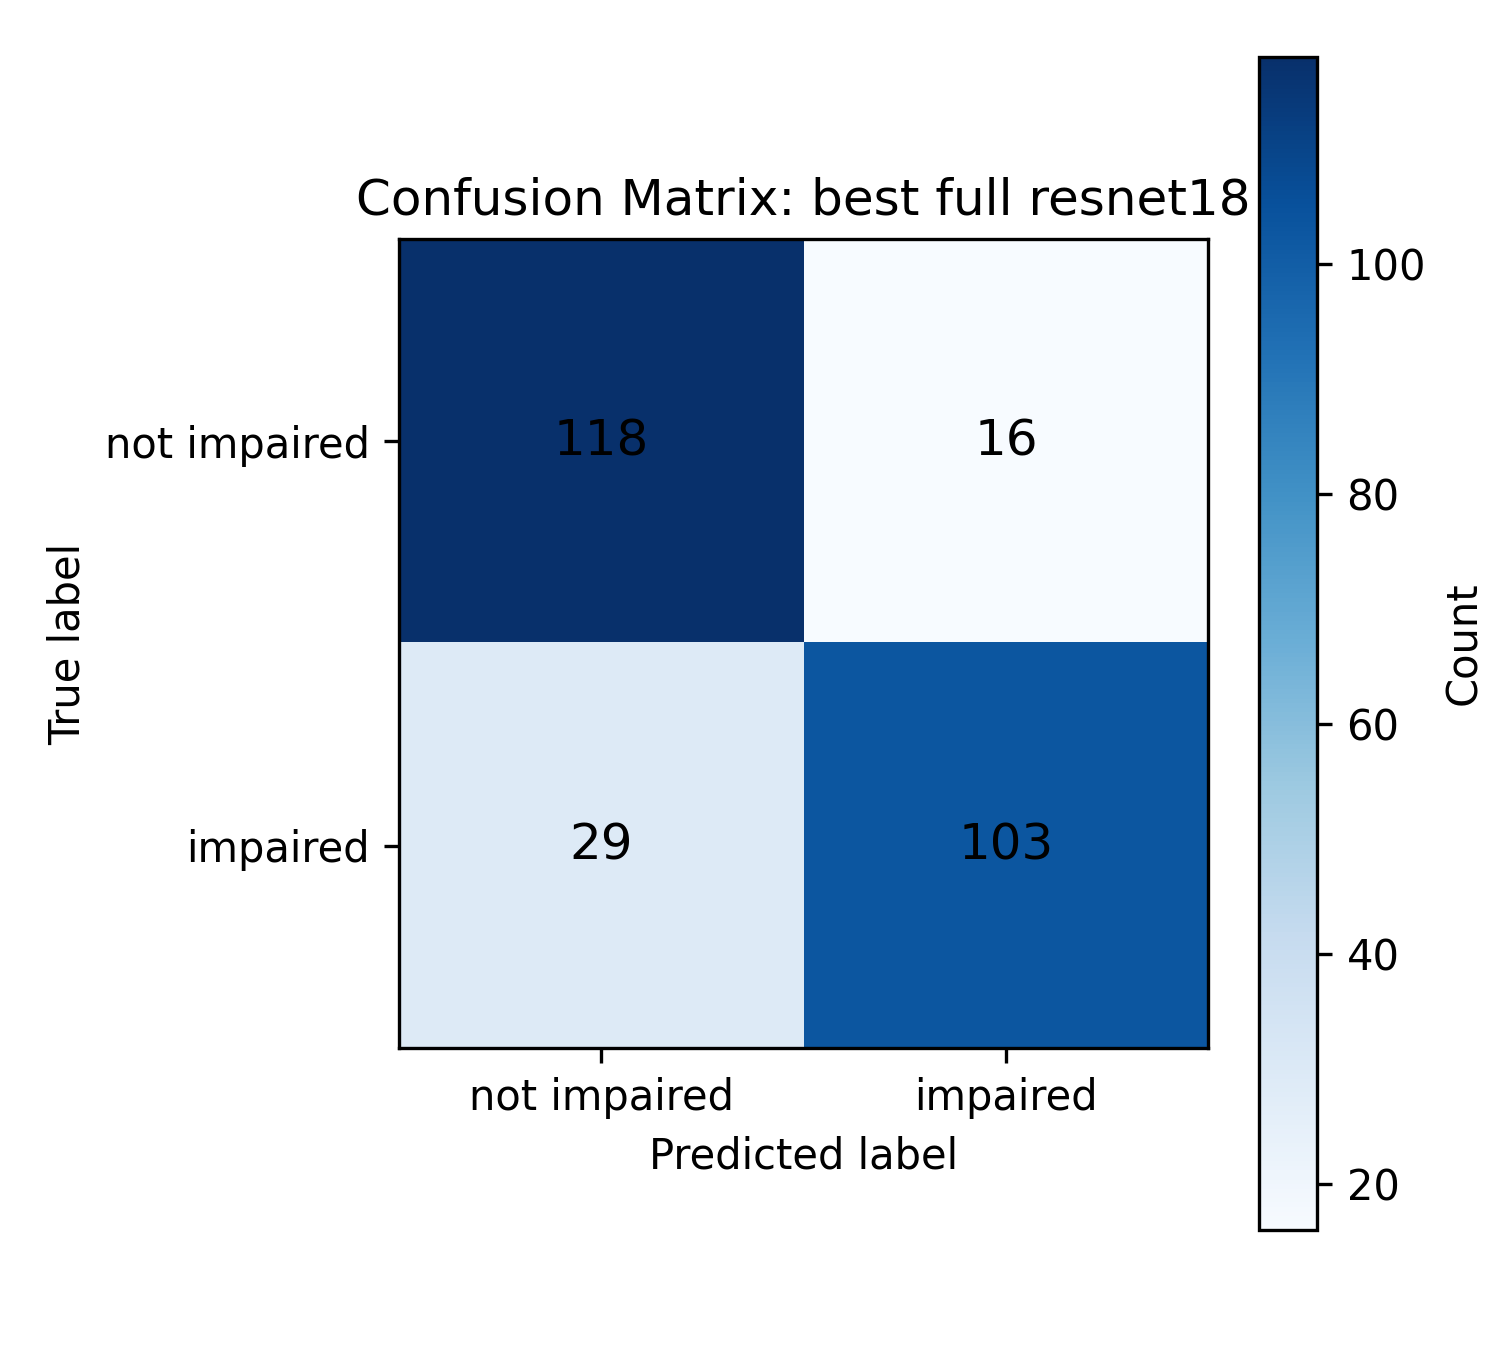
\includegraphics[width=\linewidth]{figures/diagrams/best_full_resnet18_confusion_matrix.png}
    \caption{Best full-image model.}
    \label{fig:cm-full}
  \end{subfigure}\hfill
  \begin{subfigure}[t]{0.48\linewidth}
    \centering
    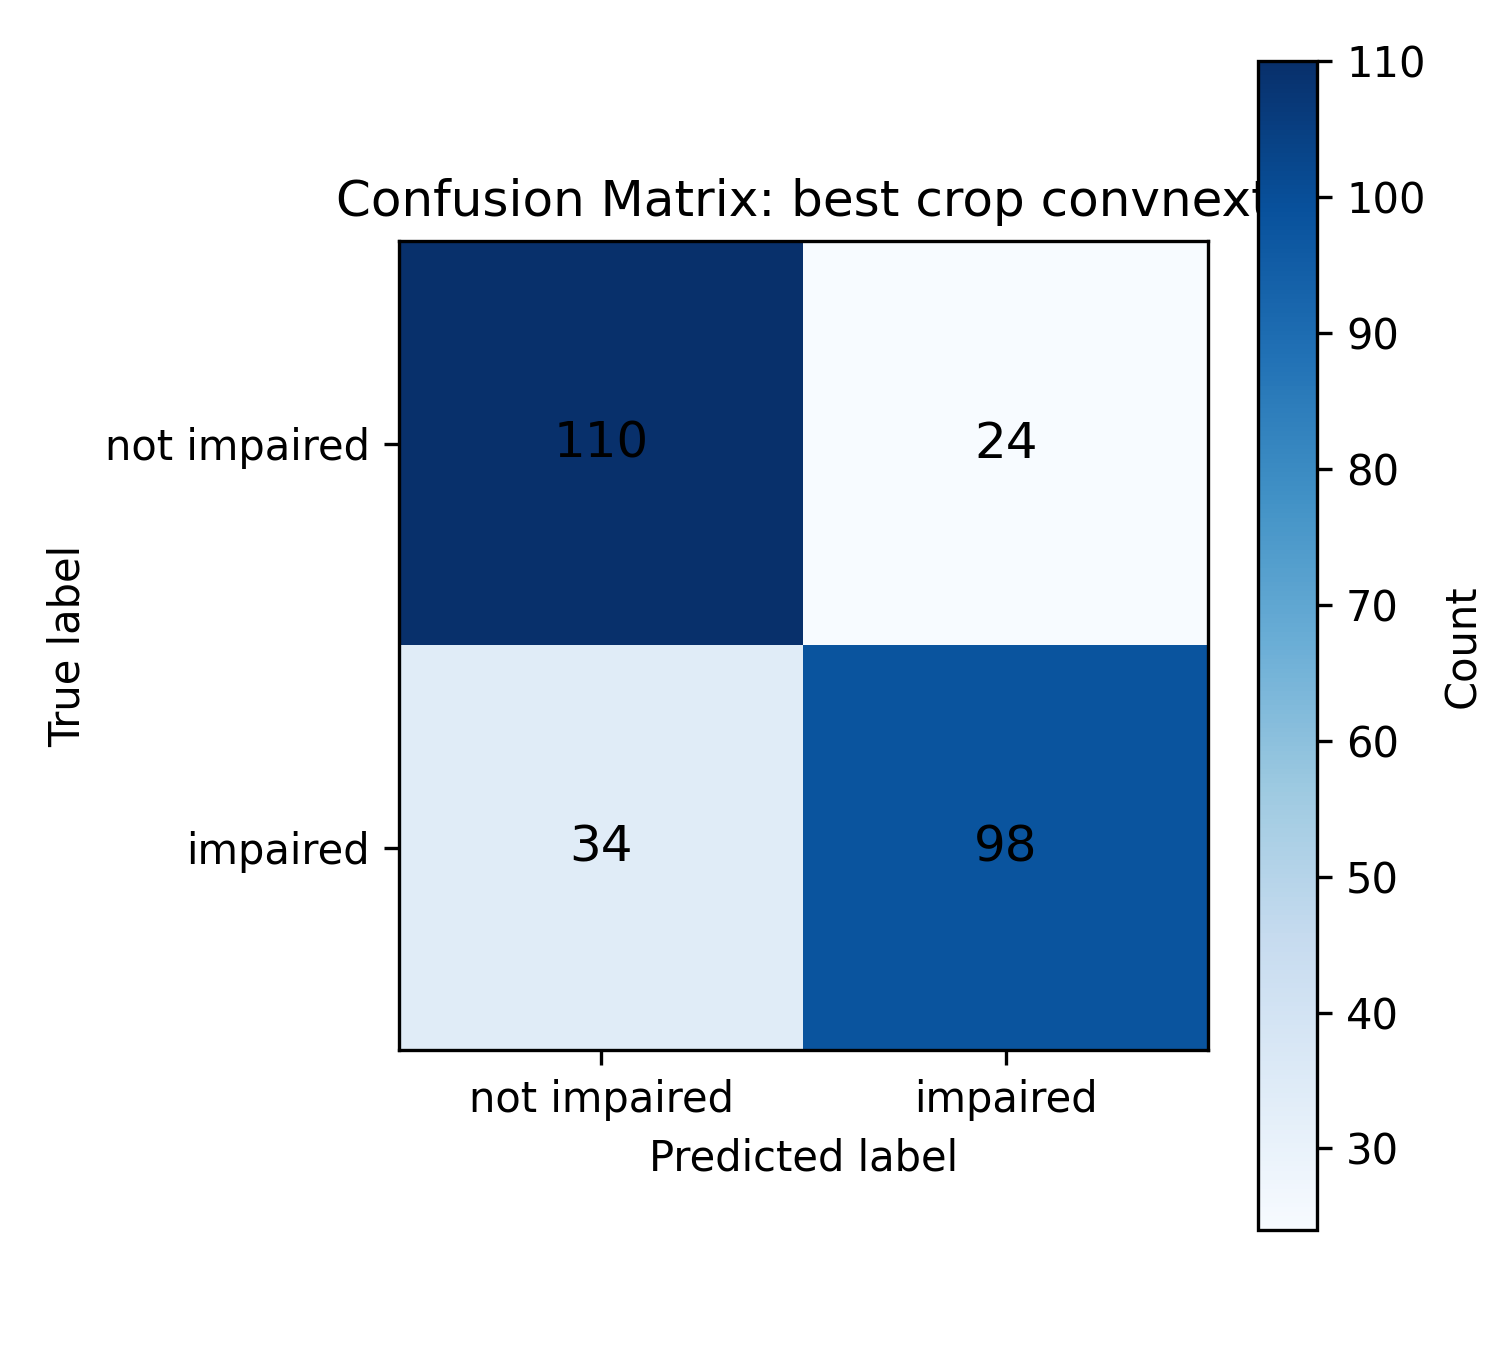
\includegraphics[width=\linewidth]{figures/diagrams/best_crop_convnext_confusion_matrix.png}
    \caption{Best crop model.}
    \label{fig:cm-crop}
  \end{subfigure}
  \caption{Confusion matrices on the held-out test set ($n=266$). Left:
  ResNet18 full-image (lr~$5\mathrm{e}{-5}$). Right: ConvNeXt-Tiny crop
  (dropout~$0.0$).}
  \label{fig:confusion}
\end{figure}

\begin{table}[t]
  \centering
  \caption{Per-class precision, recall, and F1-score for the best full-image
  and best crop models on the held-out test set.}
  \label{tab:per-class}
  \small
  \begin{tabular}{llccc}
    \toprule
    Model & Class & Prec. & Recall & F1 \\
    \midrule
    \multirow{2}{*}{\shortstack[l]{ResNet18\\(full)}}
      & not impaired & 0.803 & 0.881 & 0.840 \\
      & impaired     & 0.866 & 0.780 & 0.821 \\
    \midrule
    \multirow{2}{*}{\shortstack[l]{ConvNeXt\\(crop)}}
      & not impaired & 0.764 & 0.821 & 0.791 \\
      & impaired     & 0.803 & 0.742 & 0.772 \\
    \bottomrule
  \end{tabular}
\end{table}

The full-image ResNet18 correctly classifies $118$ of $134$ not-impaired
images (specificity $=0.881$) and $103$ of $132$ impaired images (sensitivity
$=0.780$). The crop-based ConvNeXt-Tiny shows a similar pattern---higher
specificity ($0.821$) than sensitivity ($0.742$)---but with wider margins in
both directions. In both models, the not-impaired class is easier to
recognize, which may reflect the fact that absence of grimace cues provides a
more uniform visual pattern than the diverse manifestations of impairment.

\subsection{Per-Subset Analysis}
\label{subsec:subset}

Table~\ref{tab:subset} breaks down the best full-image model's performance by
data subset. Substantial variation is visible: KH and JW achieve Macro-F1
above $0.87$, whereas AW reaches only $0.58$ despite similar balanced accuracy
being low ($0.575$).

\begin{table}[t]
  \centering
  \caption{Per-subset held-out metrics for the best full-image model (ResNet18,
  lr~$5\mathrm{e}{-5}$). $n$: number of test images.}
  \label{tab:subset}
  \small
  \begin{tabular}{lcccc}
    \toprule
    Subset & $n$ & Acc. & Bal.\ Acc. & Macro-F1 \\
    \midrule
    KH & 77 & 0.883 & 0.890 & 0.882 \\
    JW & 56 & 0.875 & 0.881 & 0.873 \\
    LW & 34 & 0.941 & 0.800 & 0.858 \\
    MR & 86 & 0.744 & 0.745 & 0.744 \\
    AW & 13 & 0.615 & 0.575 & 0.575 \\
    \bottomrule
  \end{tabular}
\end{table}

AW's poor performance likely stems from its very small test partition ($n=13$,
of which only $5$ are impaired) and potentially distinct imaging conditions.
MR, despite being the largest subset ($n=86$), also underperforms the global
average, suggesting systematic differences in recording setup or animal
strain. The high accuracy of LW ($0.941$) is notable but must be interpreted
cautiously: this subset is heavily imbalanced toward not-impaired ($29$ vs.\
$5$), inflating accuracy while balanced accuracy ($0.800$) and Macro-F1
($0.858$) are lower.

\subsection{Training Curves}
\label{subsec:diagrams}

Figure~\ref{fig:train-curves} shows train/validation loss, accuracy, and
Macro-F1 for the best crop and best full-image models. Training metrics
approach near-perfect values while validation Macro-F1 plateaus, and
validation loss rises later in training, indicating overfitting despite early
stopping on validation Macro-F1.

\begin{figure*}[htbp]
  \centering
  \begin{subfigure}[t]{0.98\textwidth}
    \centering
    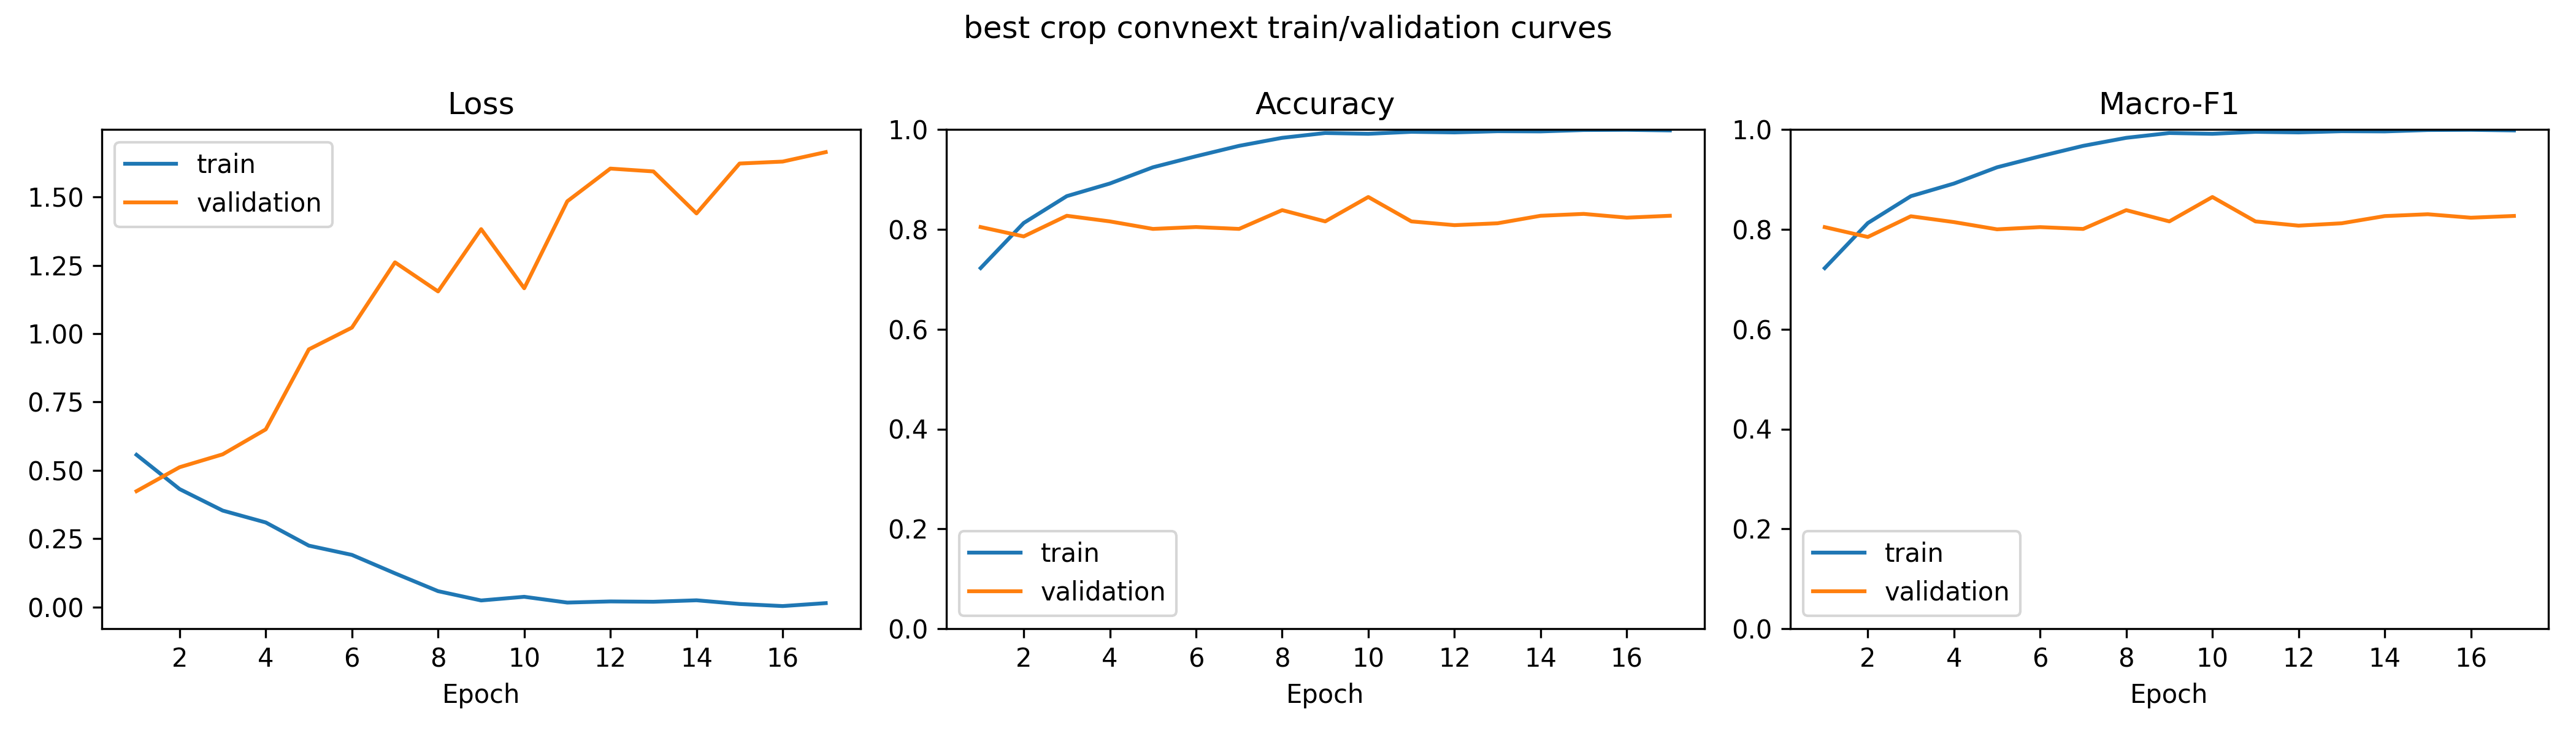
\includegraphics[width=0.95\linewidth]{figures/diagrams/best_crop_convnext_train_val_curves.png}
    \caption{Best crop model (ConvNeXt-Tiny, light augmentation, dropout $0.0$).}
    \label{fig:curve-crop}
  \end{subfigure}

  \vspace{0.4em}

  \begin{subfigure}[t]{0.98\textwidth}
    \centering
    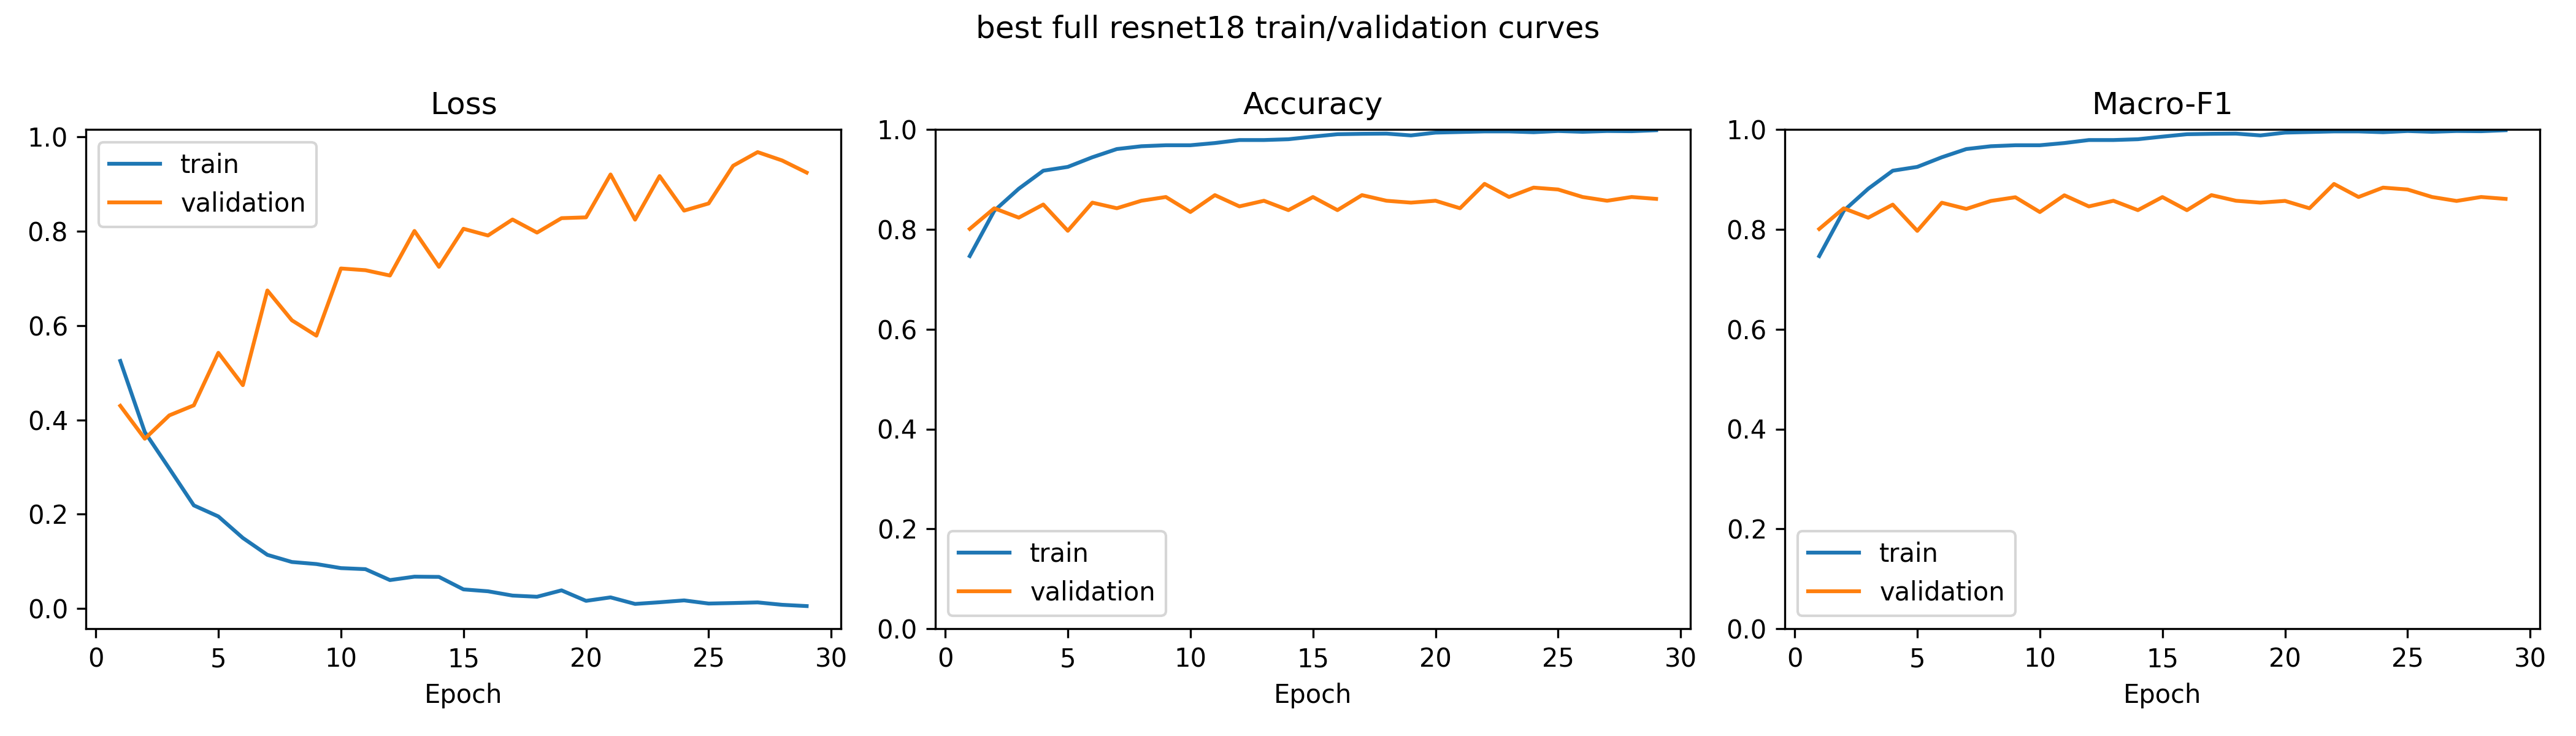
\includegraphics[width=0.95\linewidth]{figures/diagrams/best_full_resnet18_train_val_curves.png}
    \caption{Best full-image model (ResNet18, light augmentation, lr $5\mathrm{e}{-5}$).}
    \label{fig:curve-full}
  \end{subfigure}
  \caption{Training and validation curves for the best crop and full-image
  configurations. Validation loss increases after the best checkpoint epoch,
  indicating overfitting; early stopping restores the highest-F1 checkpoint.}
  \label{fig:train-curves}
\end{figure*}

\subsection{Prediction Confidence and Threshold Sensitivity}
\label{subsec:threshold}

Figure~\ref{fig:prob-hist} shows the distribution of predicted impaired-class
probabilities for both best models. Both histograms are strongly bimodal:
most test samples receive predictions near $0.0$ or near $1.0$, with few
samples in the uncertain region around $0.5$. This indicates that the models
are generally confident, and that the fixed threshold of $0.5$ falls in a
natural separation region.

Figure~\ref{fig:threshold-curves} displays threshold sensitivity curves for
both best models. Macro-F1 remains remarkably stable across a wide range of
thresholds (approximately $0.2$ to $0.7$), varying by less than $3$~pp. This
robustness suggests that the models' discriminative power is not an artifact
of threshold tuning, and that the default threshold of $0.5$ is a reasonable
choice even without validation-based optimization.

\begin{figure}[htbp]
  \centering
  \begin{subfigure}[t]{0.48\linewidth}
    \centering
    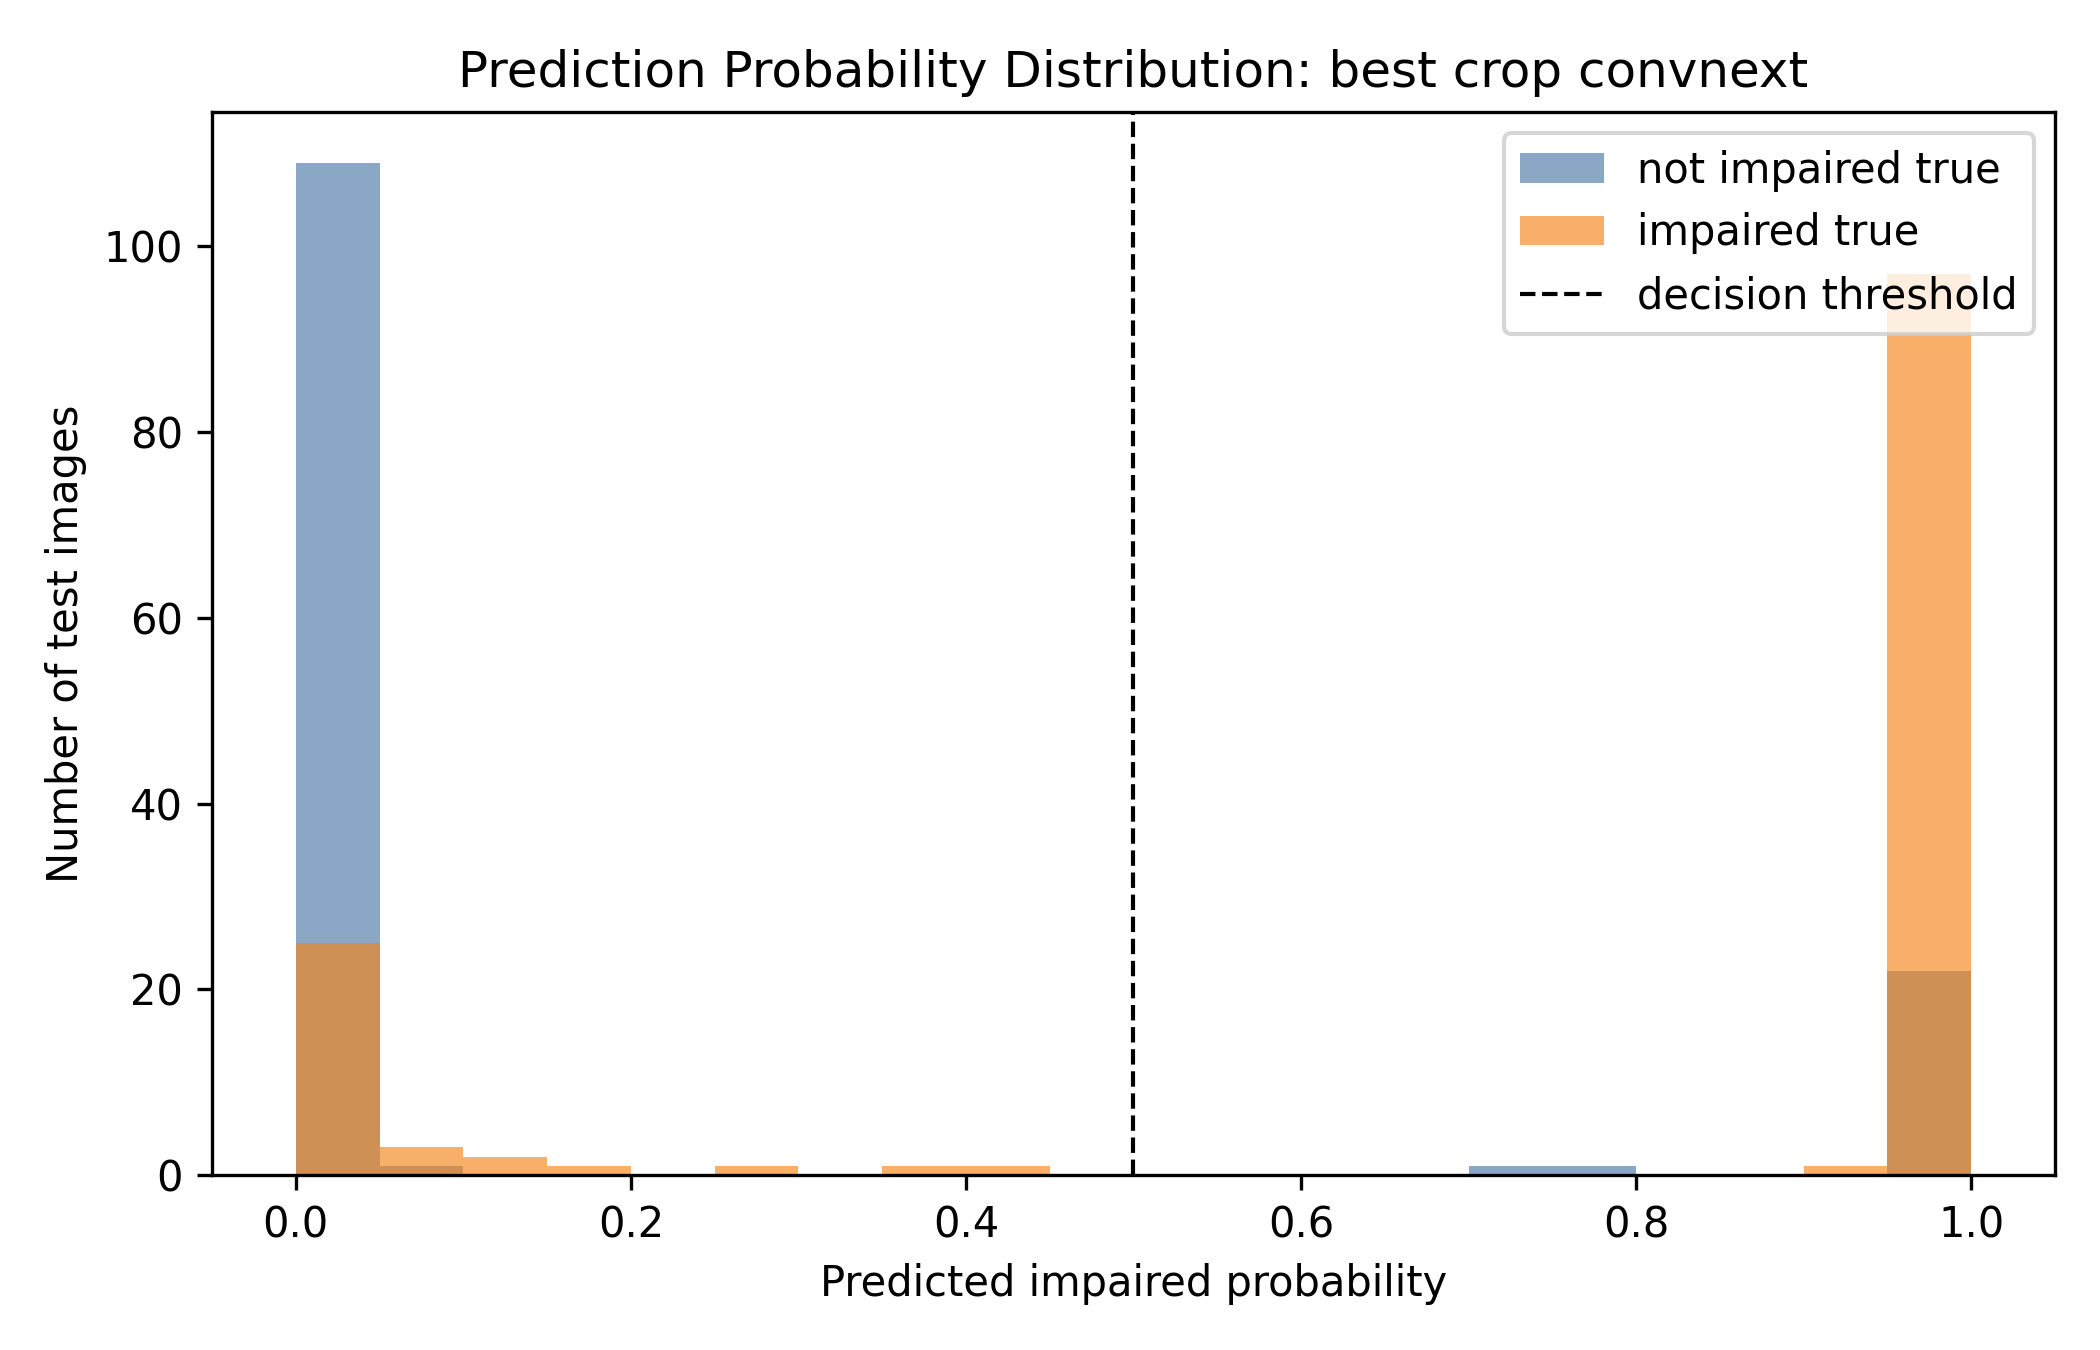
\includegraphics[width=\linewidth]{figures/diagrams/best_crop_convnext_probability_histogram.png}
    \caption{Best crop model.}
    \label{fig:prob-crop}
  \end{subfigure}\hfill
  \begin{subfigure}[t]{0.48\linewidth}
    \centering
    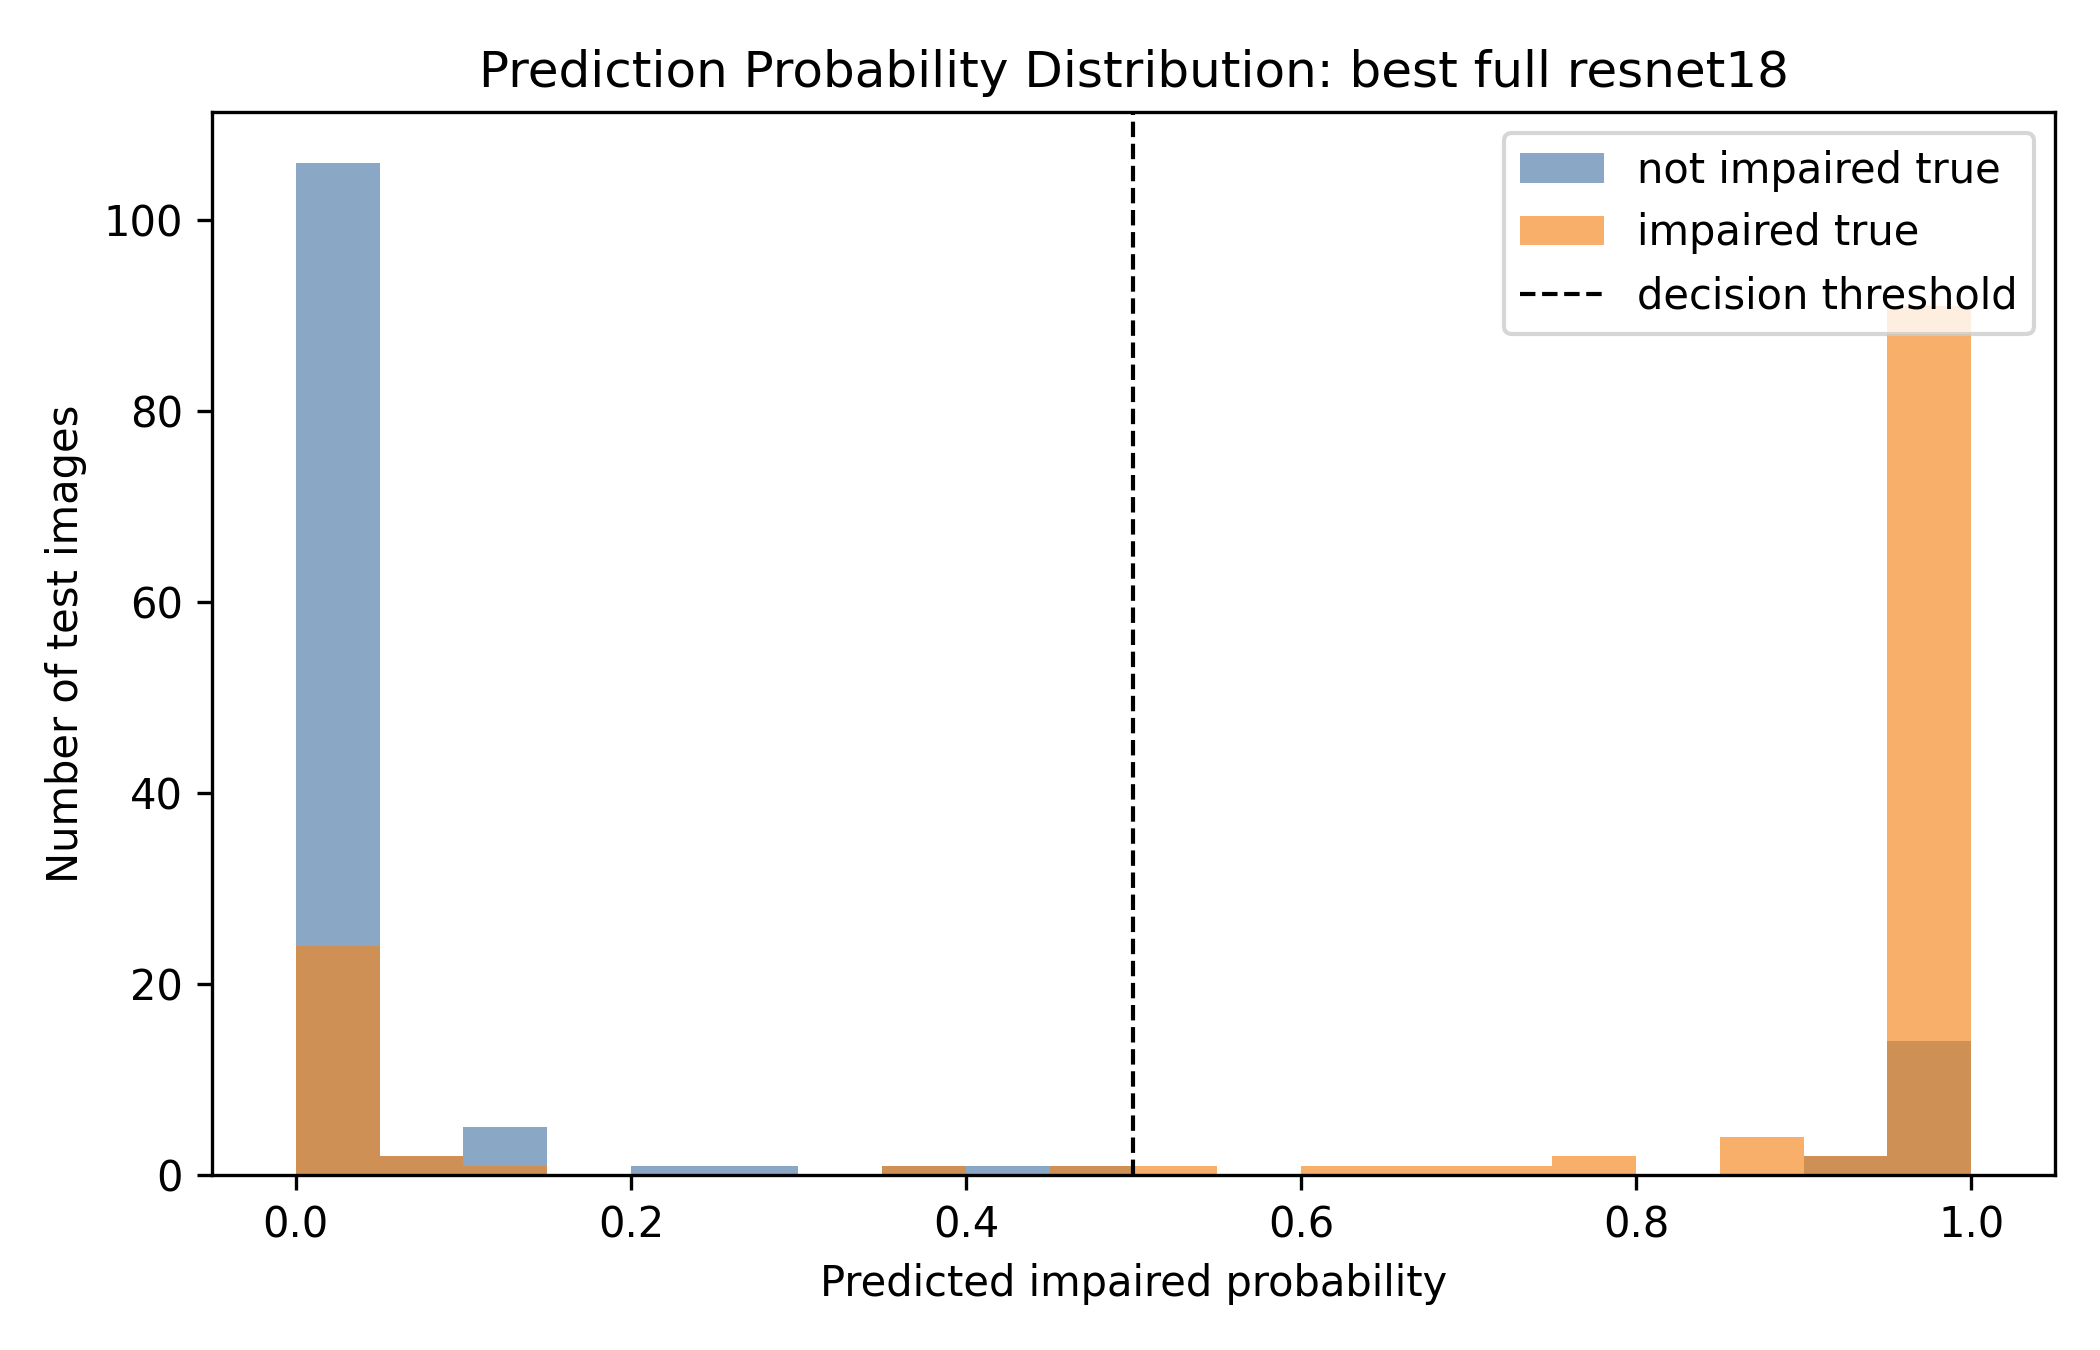
\includegraphics[width=\linewidth]{figures/diagrams/best_full_resnet18_probability_histogram.png}
    \caption{Best full-image model.}
    \label{fig:prob-full}
  \end{subfigure}
  \caption{Prediction probability distributions for the impaired class on the
  held-out test set. The bimodal separation indicates high confidence for most
  predictions.}
  \label{fig:prob-hist}
\end{figure}

\begin{figure}[htbp]
  \centering
  \begin{subfigure}[t]{0.48\linewidth}
    \centering
    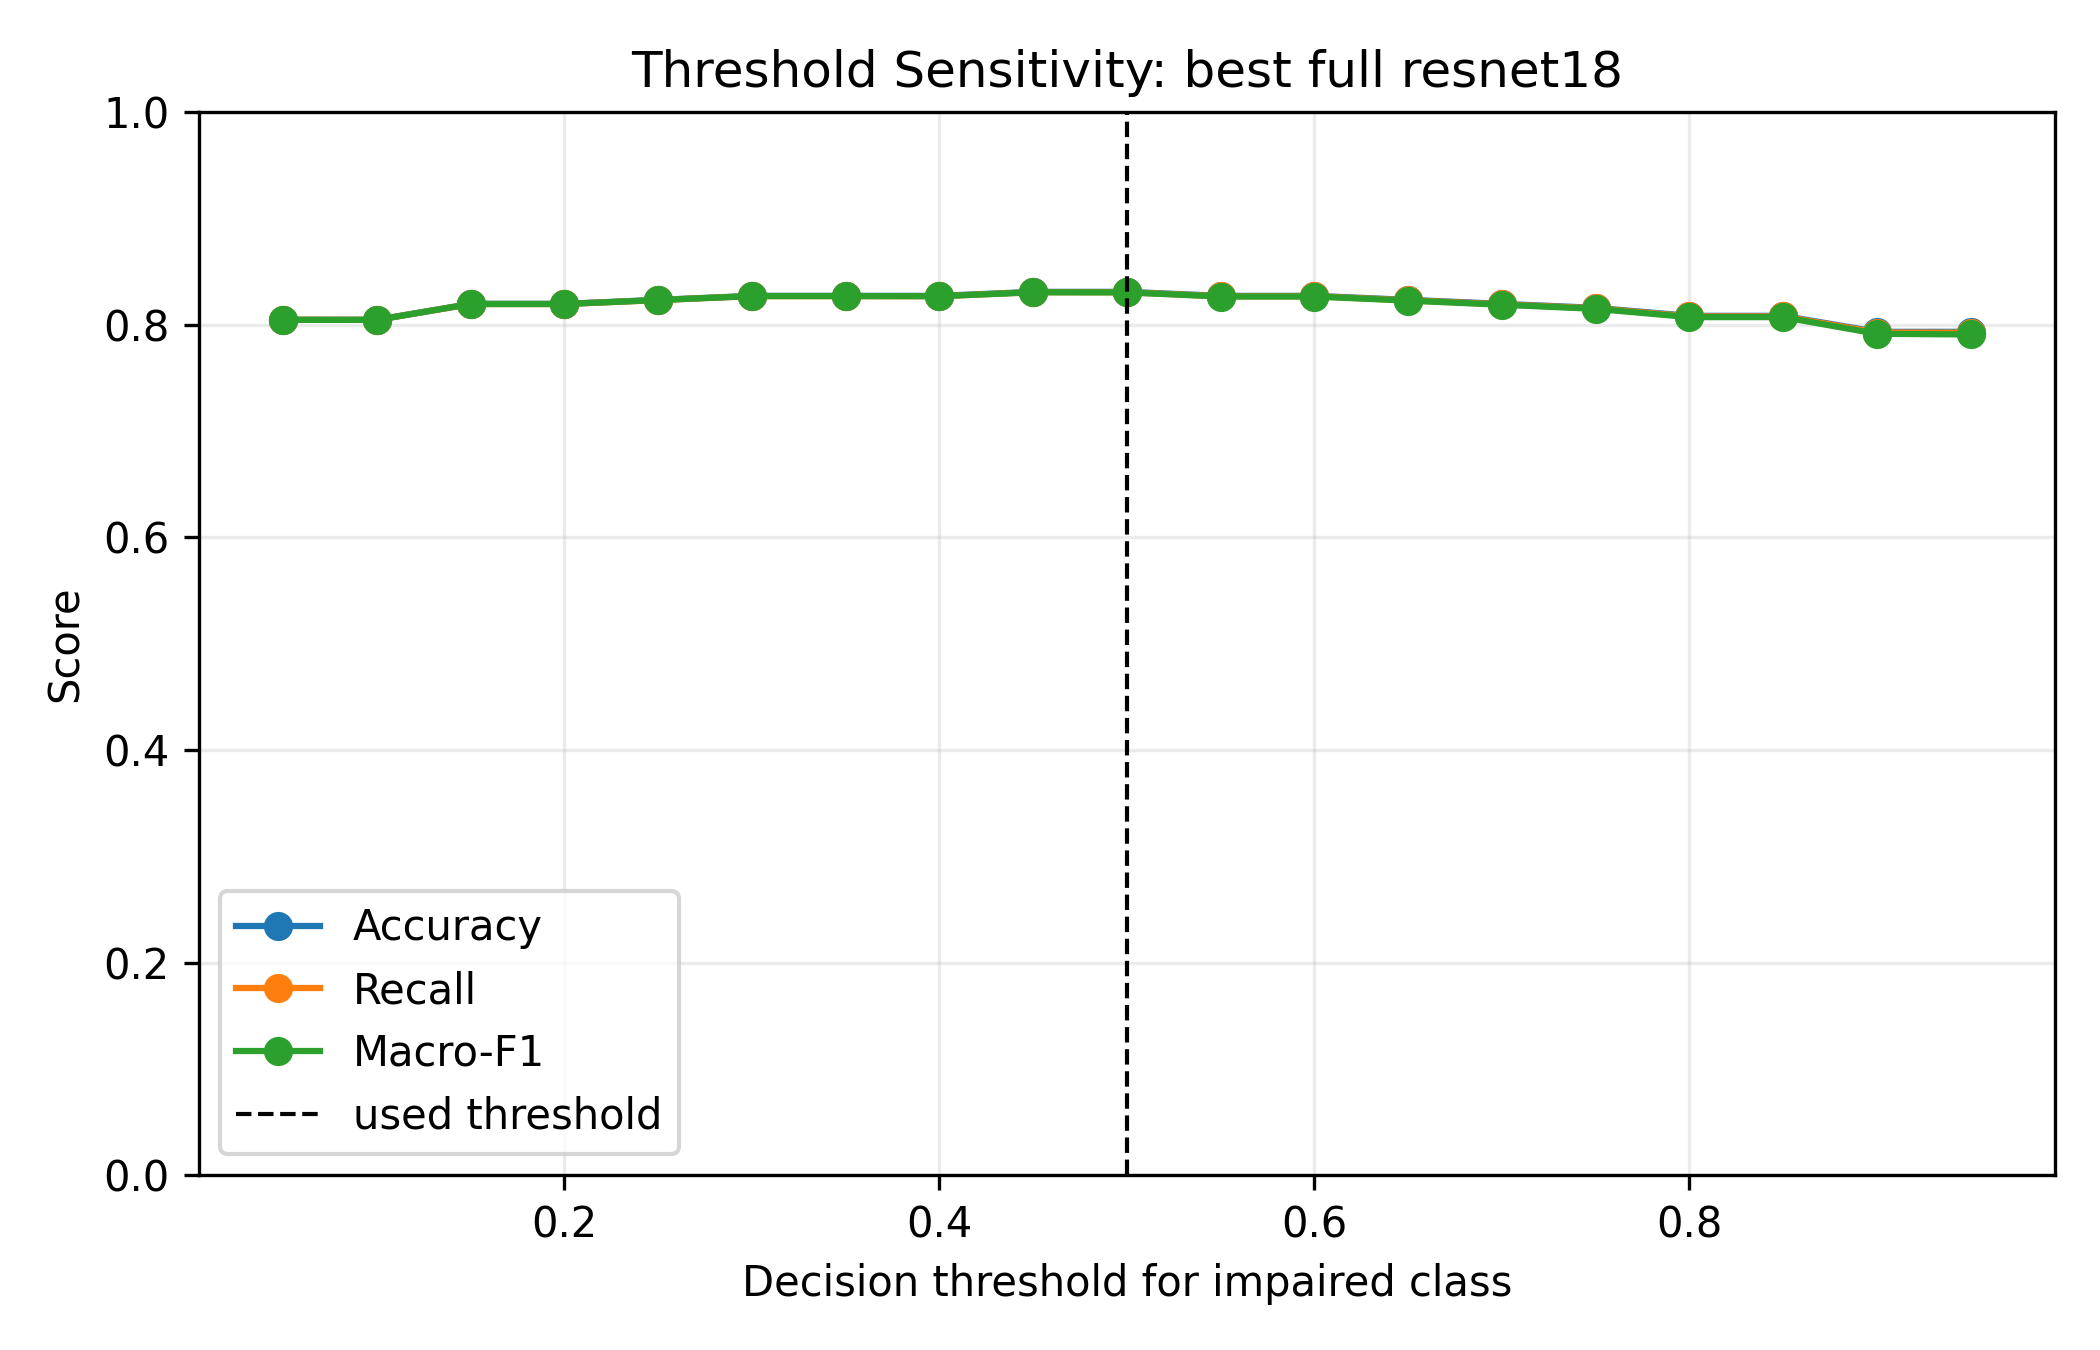
\includegraphics[width=\linewidth]{figures/diagrams/best_full_resnet18_threshold_curve.png}
    \caption{Best full-image model.}
    \label{fig:thresh-full}
  \end{subfigure}\hfill
  \begin{subfigure}[t]{0.48\linewidth}
    \centering
    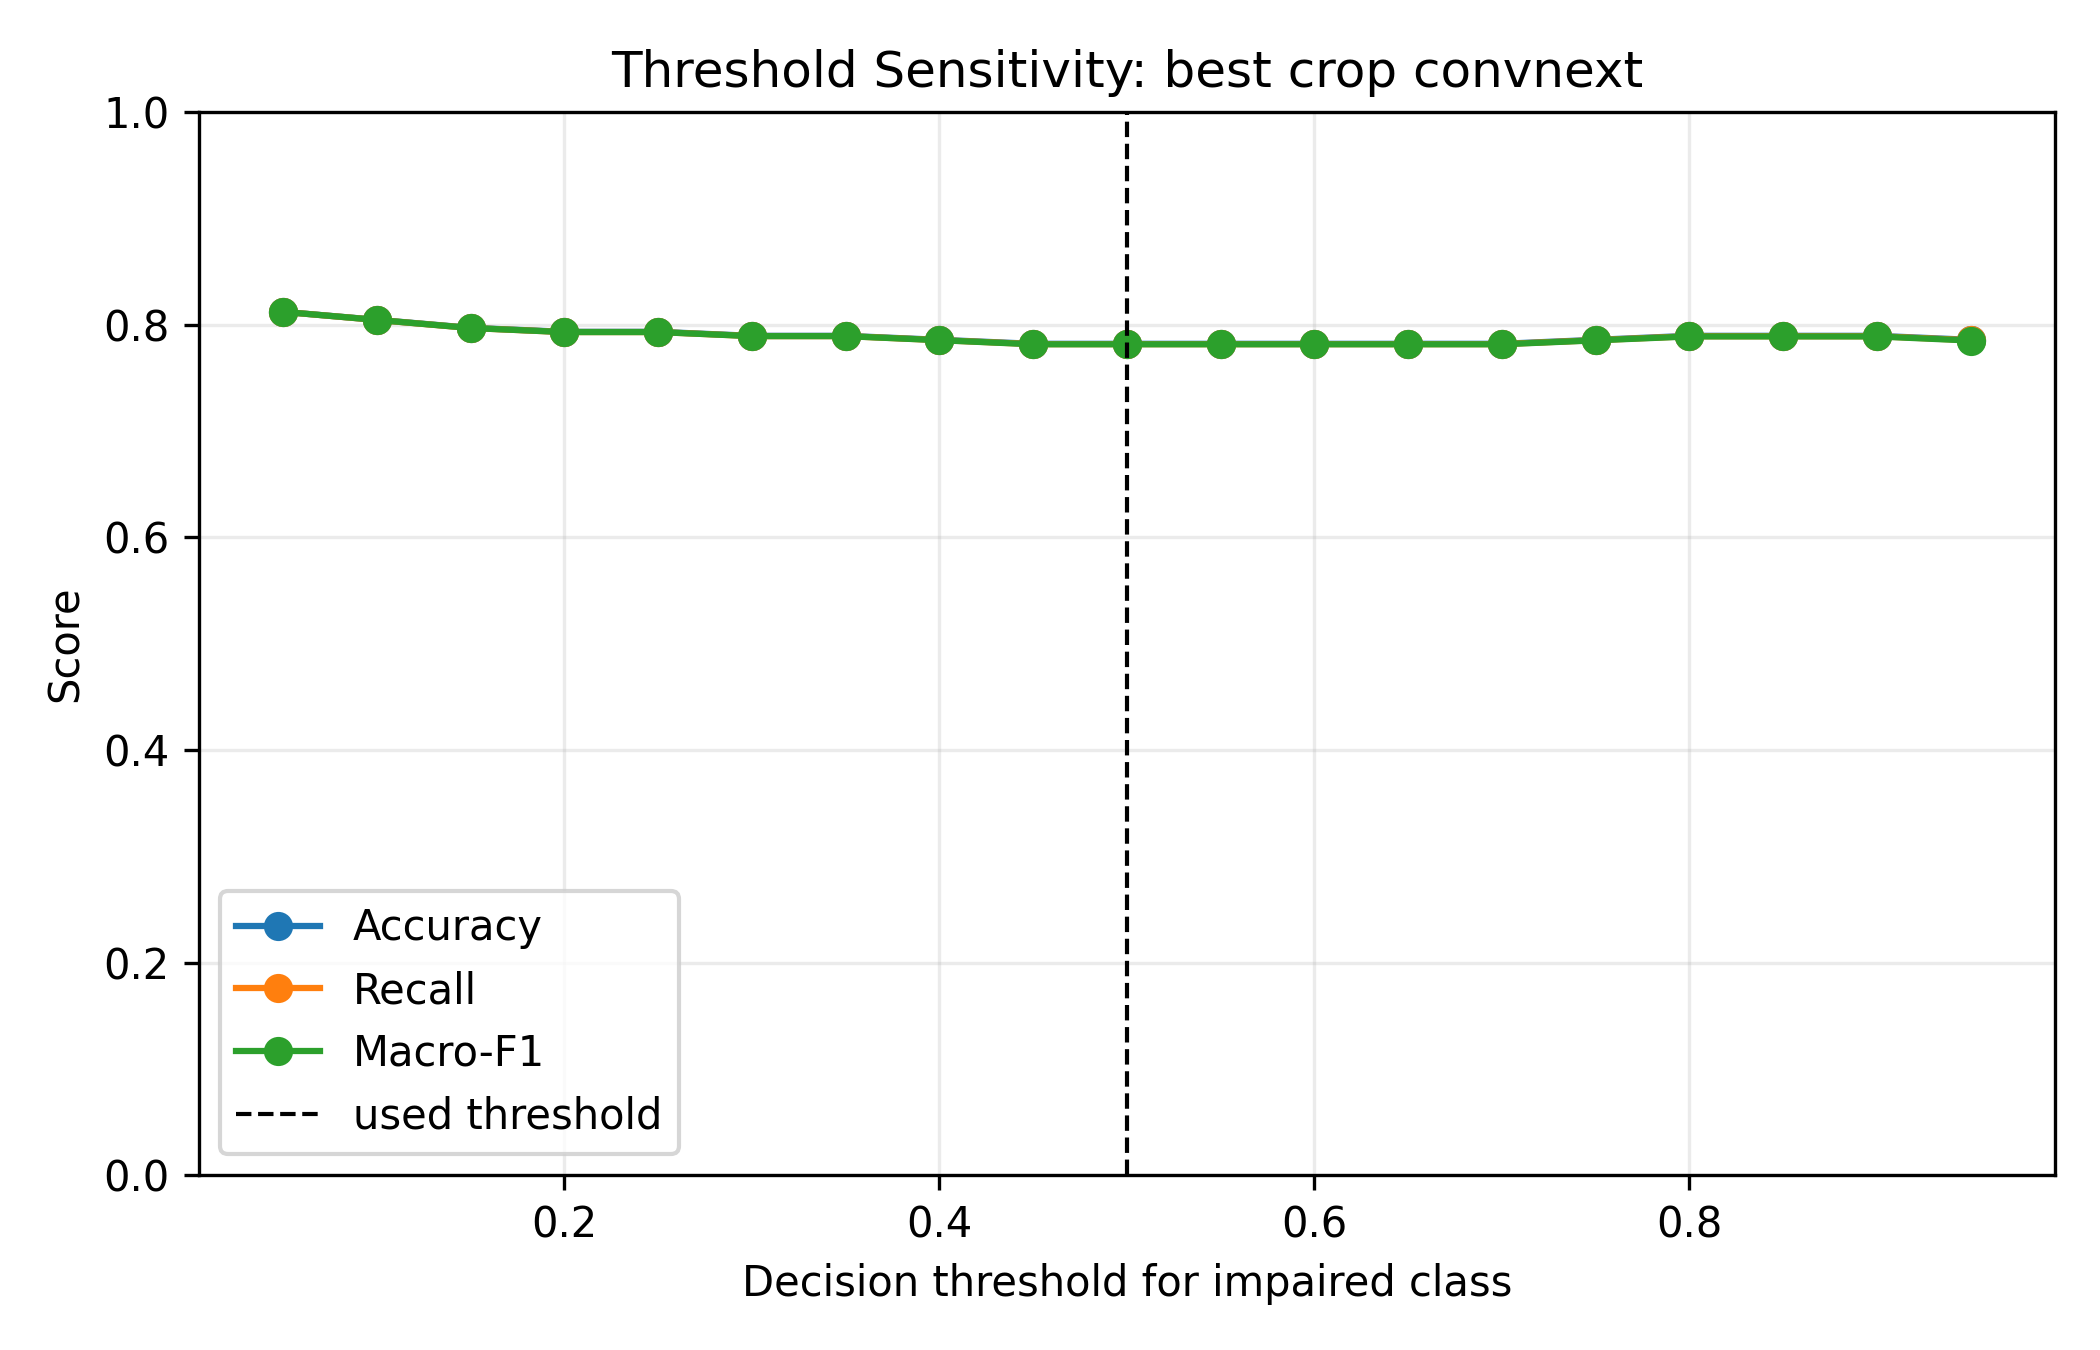
\includegraphics[width=\linewidth]{figures/diagrams/best_crop_convnext_threshold_curve.png}
    \caption{Best crop model.}
    \label{fig:thresh-crop}
  \end{subfigure}
  \caption{Threshold sensitivity: Macro-F1 versus the impaired-class decision
  threshold. Both models are stable across a broad threshold range.}
  \label{fig:threshold-curves}
\end{figure}

\subsection{Summary Comparison}
\label{subsec:summary-comparison}

Figure~\ref{fig:metric-comparison} provides a ranked overview of all
experimental runs across both parts. Figure~\ref{fig:input-type} summarizes
mean metrics aggregated by input type, confirming the overall advantage of
full-image inputs while demonstrating that the gap is modest.

\begin{figure}[htbp]
  \centering
  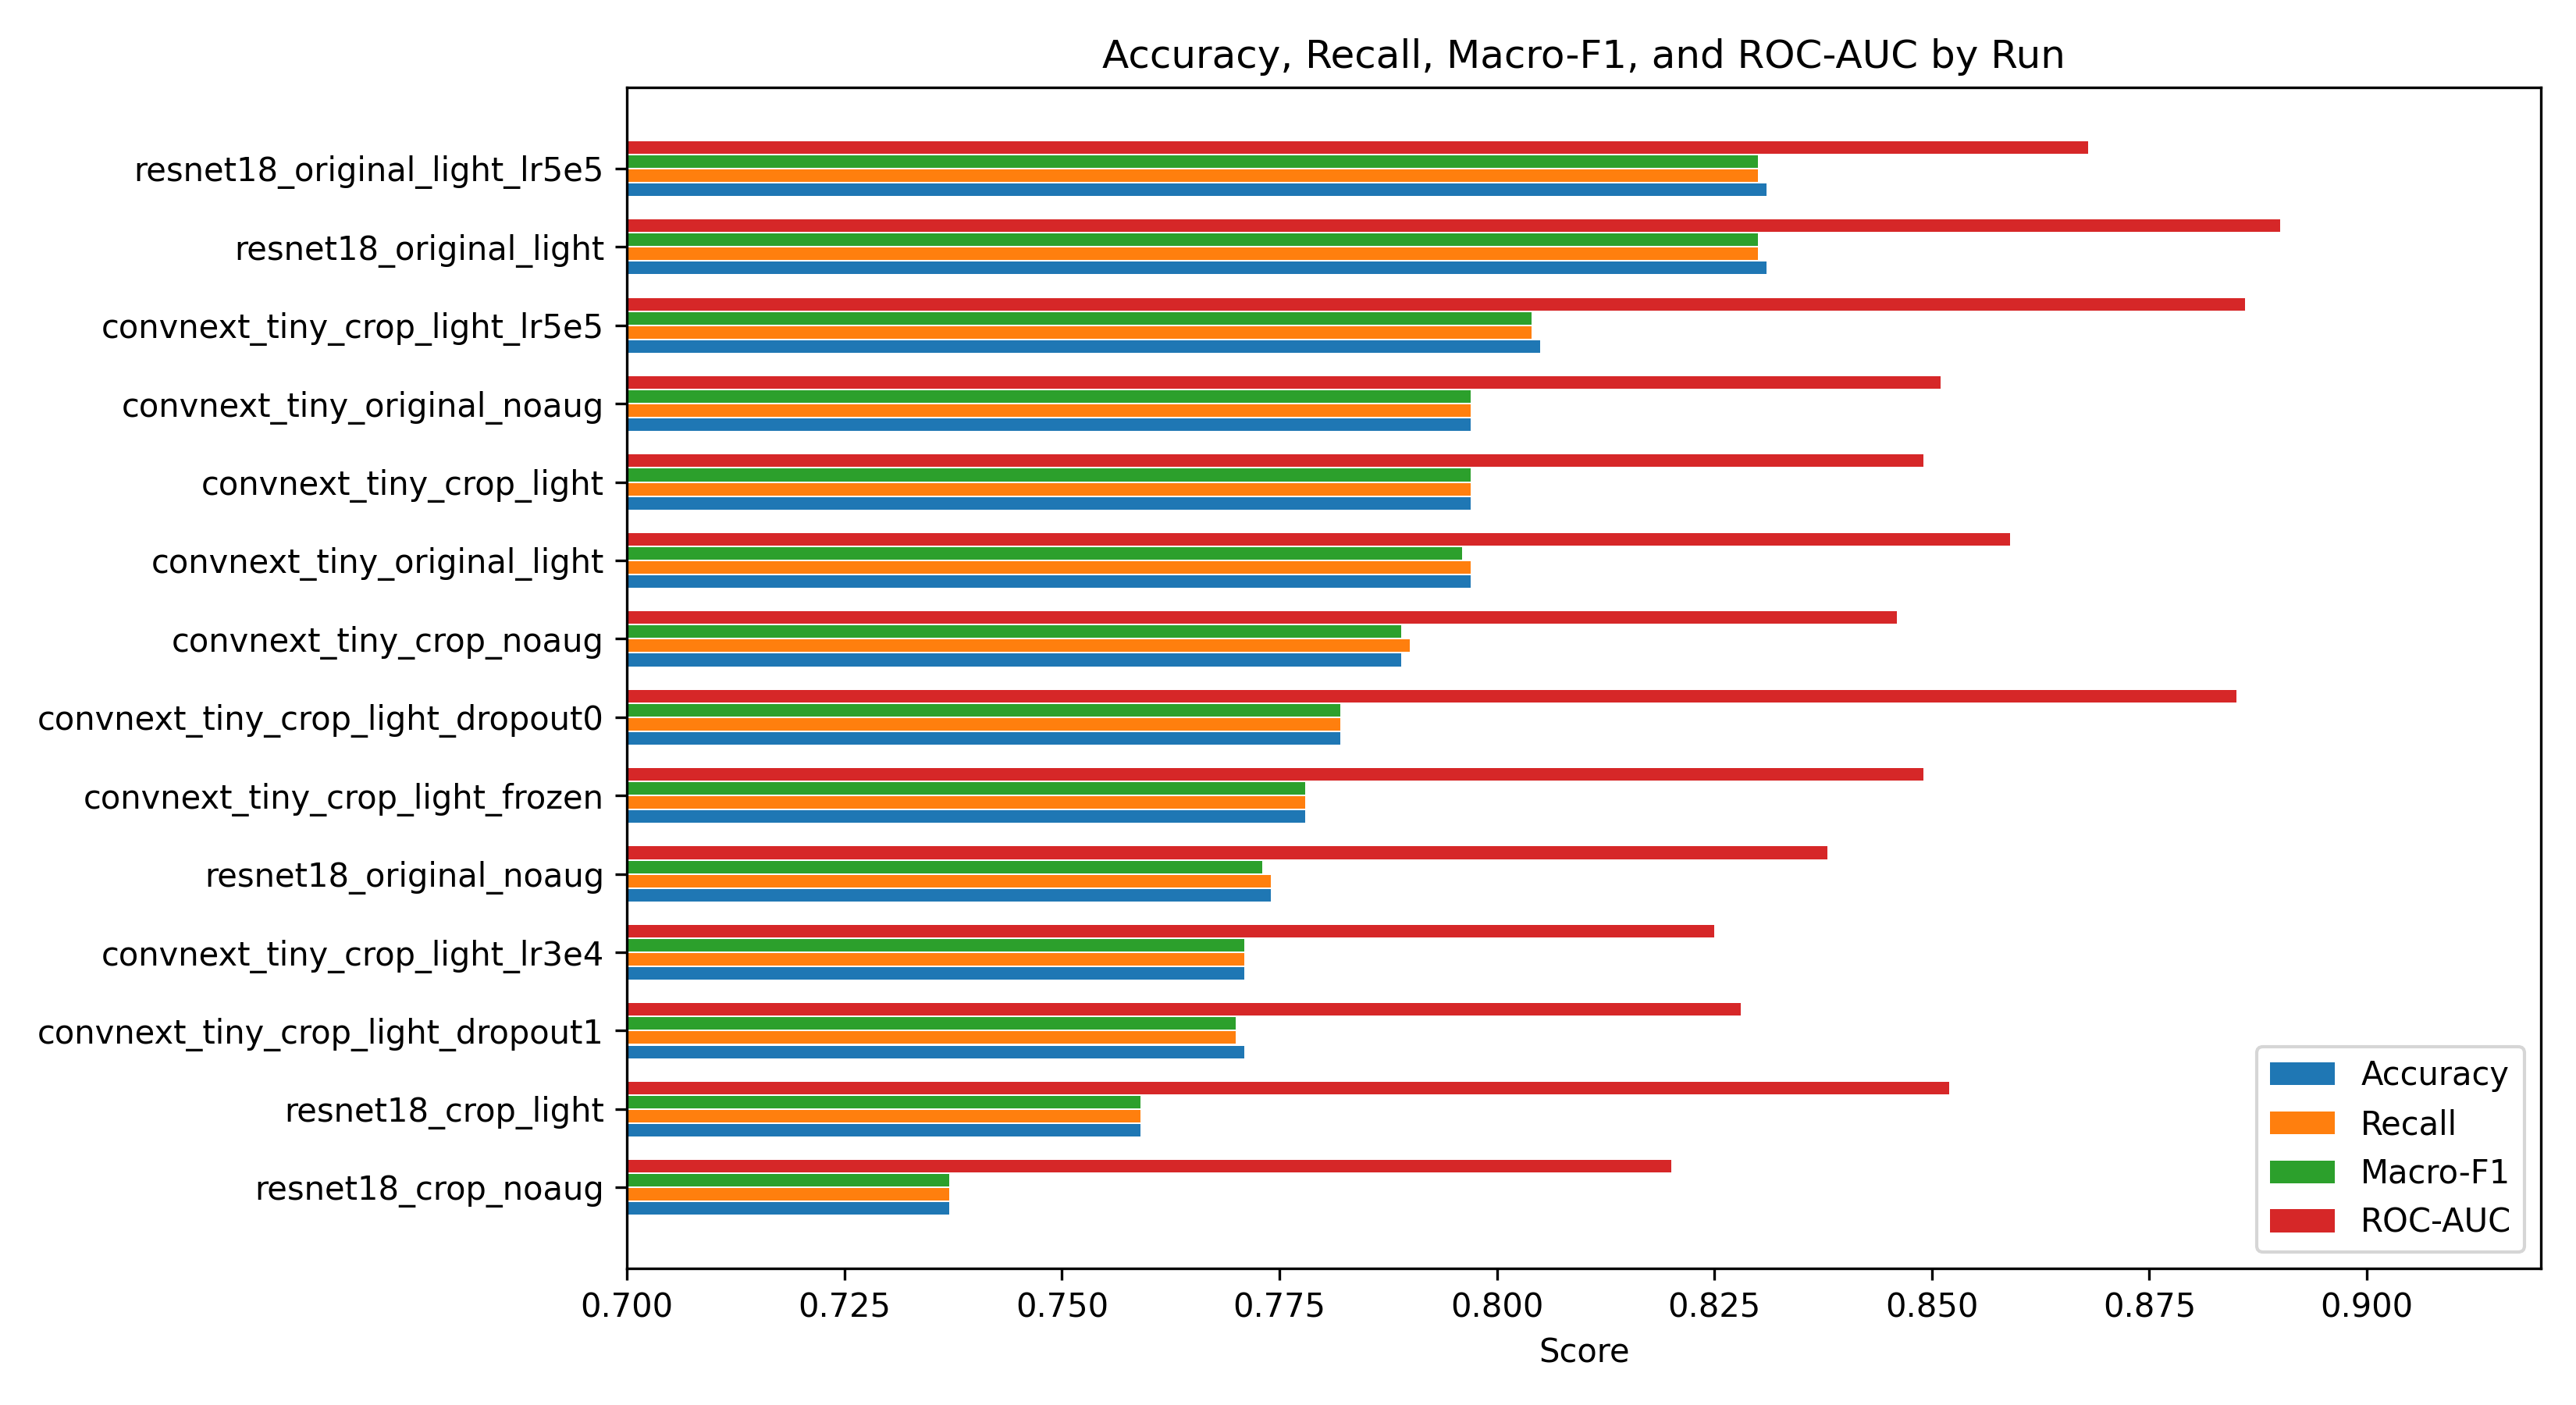
\includegraphics[width=0.95\linewidth]{figures/diagrams/all_runs_metric_comparison.png}
  \caption{Held-out Accuracy, Recall, Macro-F1, and ROC-AUC for all
  experimental runs, ranked by Macro-F1.}
  \label{fig:metric-comparison}
\end{figure}

\begin{figure}[htbp]
  \centering
  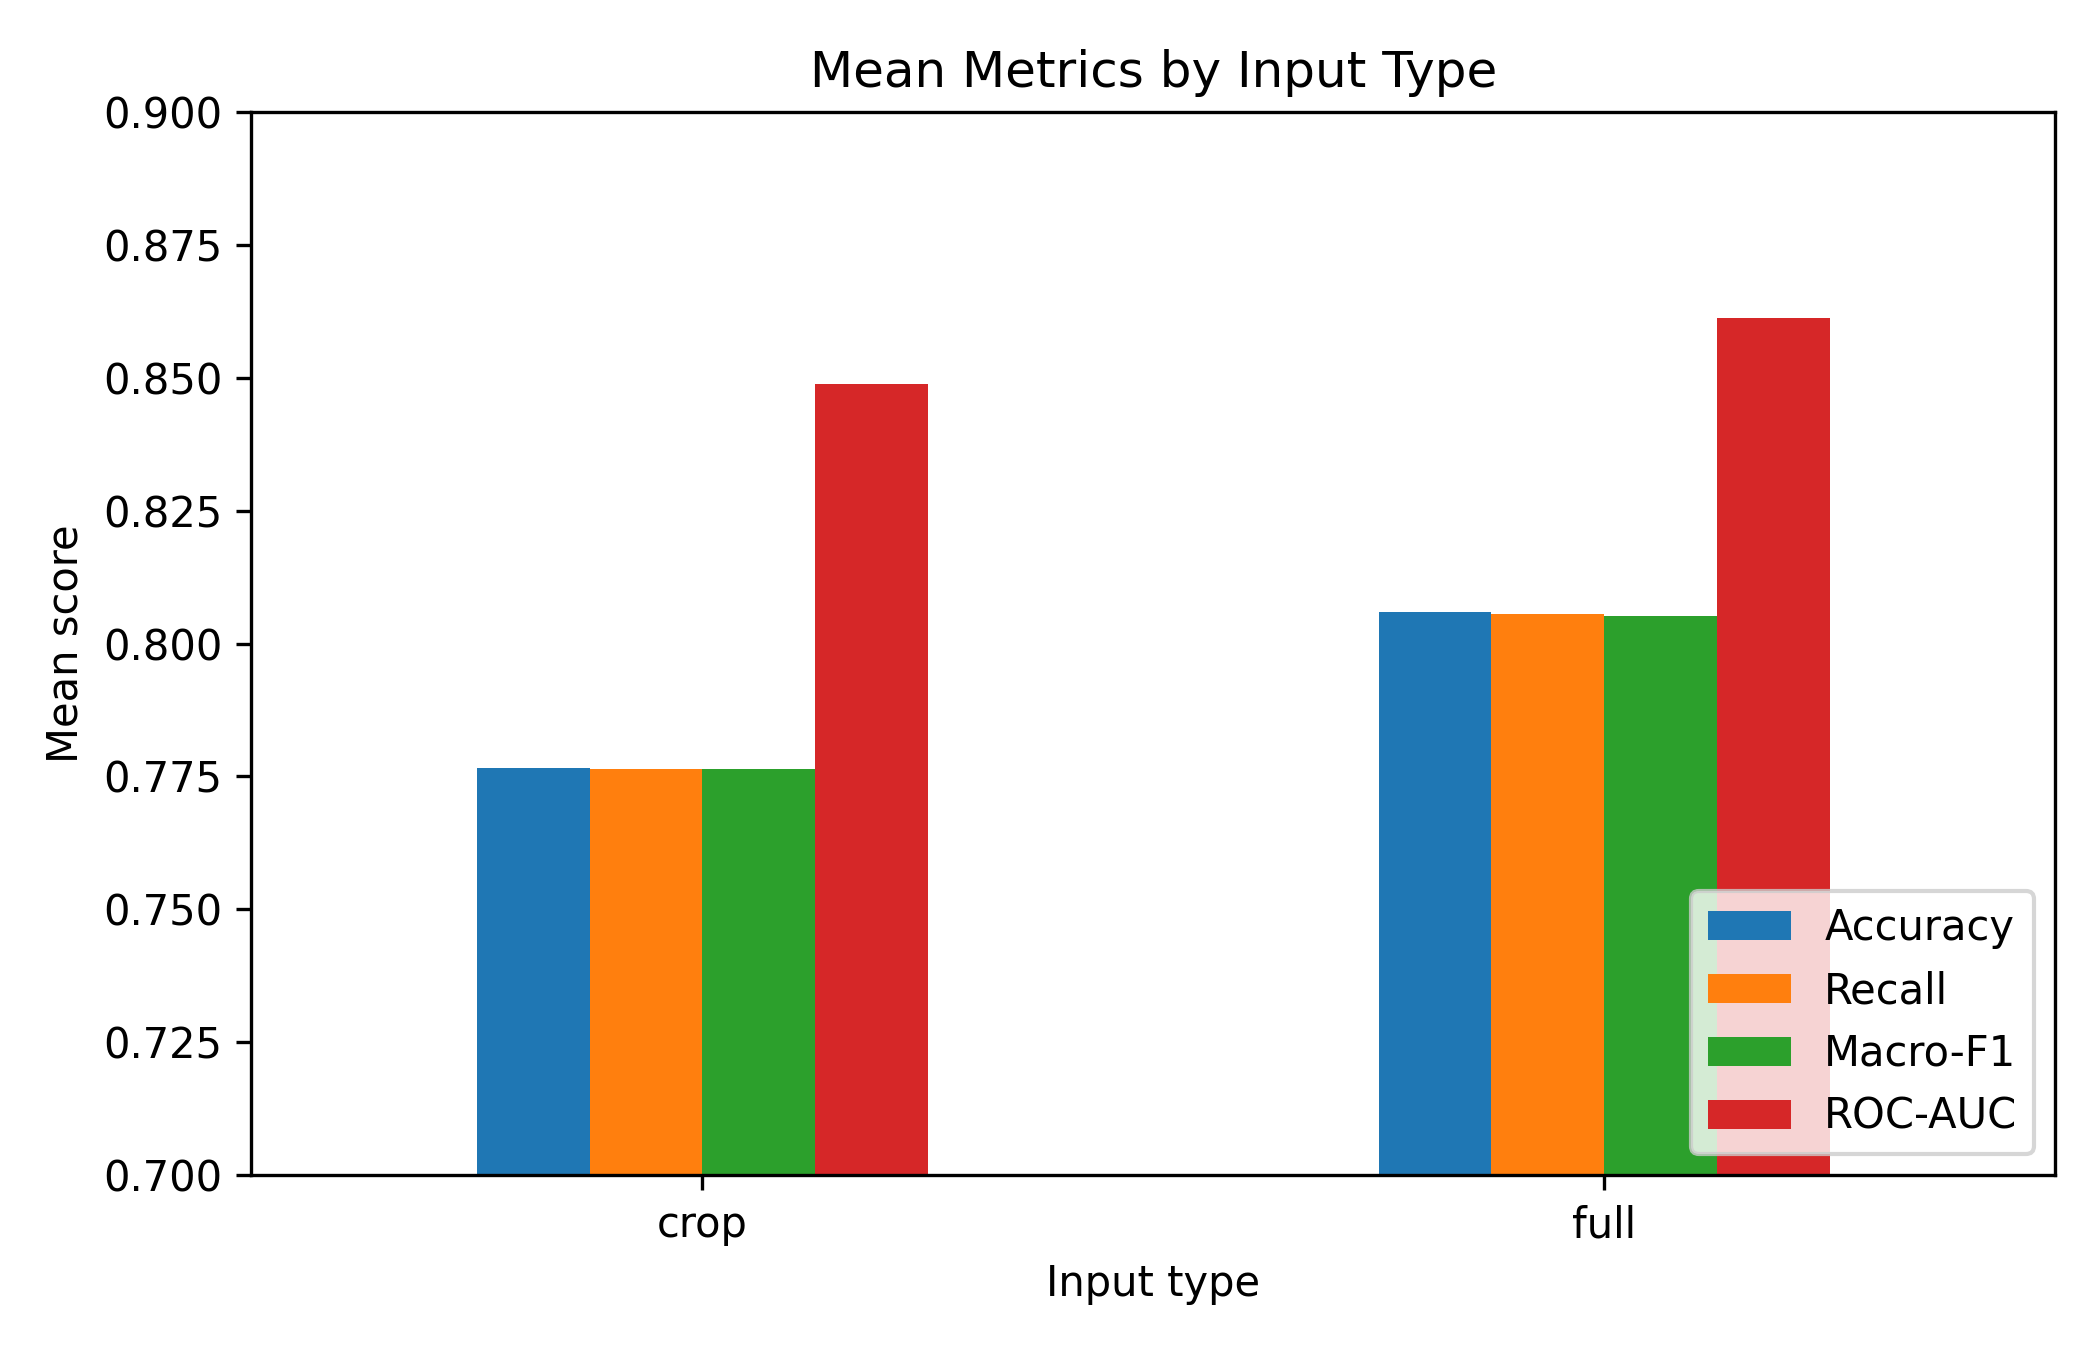
\includegraphics[width=0.75\linewidth]{figures/diagrams/mean_metrics_by_input_type.png}
  \caption{Mean held-out metrics aggregated by input type (muzzle crop vs.\
  full image).}
  \label{fig:input-type}
\end{figure}

\subsection{Qualitative Examples}
\label{subsec:qualitative}

Figure~\ref{fig:qualitative} shows representative correct and incorrect
predictions with their corresponding interpretability overlays. Each panel
pairs the input image with either a Grad-CAM heatmap or gradient-saliency
map computed for the predicted class.

For correctly classified crop images (Figures~\ref{fig:q-crop-tn}
and~\ref{fig:q-crop-tn-gc}), saliency concentrates on the muzzle tip and
whisker base---regions corresponding to the nose-bulge and whisker-change
action units of the MGS. For correctly classified full-image impaired cases
(Figures~\ref{fig:q-full-tp} and~\ref{fig:q-full-tp-gc}), Grad-CAM
highlights the cheek and periorbital regions, consistent with the
cheek-bulge and orbital-tightening MGS action units. Among
misclassified cases (Figures~\ref{fig:q-crop-fp}--\ref{fig:q-full-fn-sal}),
the models still attend to facial regions, suggesting that errors arise
from ambiguous expressions or challenging pose and lighting rather
than from attention to irrelevant background features.

\begin{figure*}[htbp]
  \centering
  \begin{subfigure}[t]{0.32\textwidth}
    \centering
    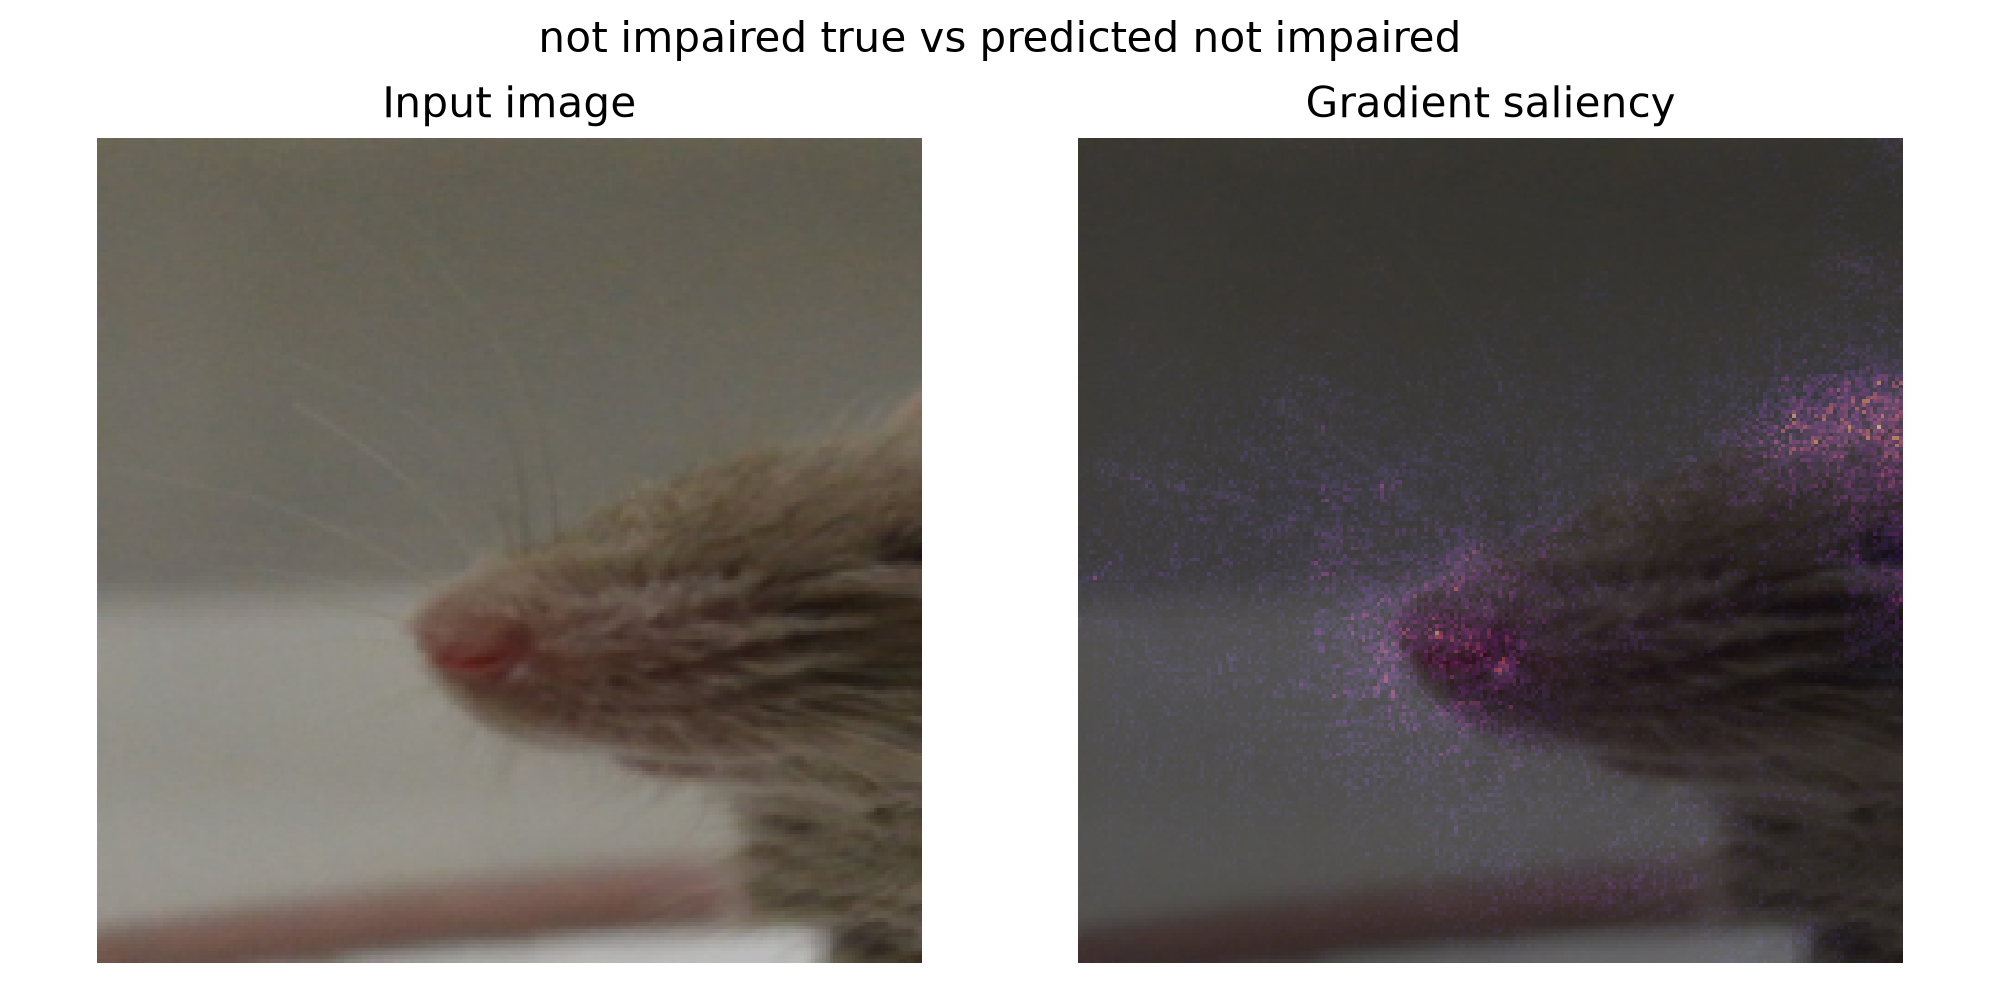
\includegraphics[width=\linewidth]{figures/qualitative/crop_tn_saliency.png}
    \caption{Crop, correct not-impaired (saliency).}
    \label{fig:q-crop-tn}
  \end{subfigure}\hfill
  \begin{subfigure}[t]{0.32\textwidth}
    \centering
    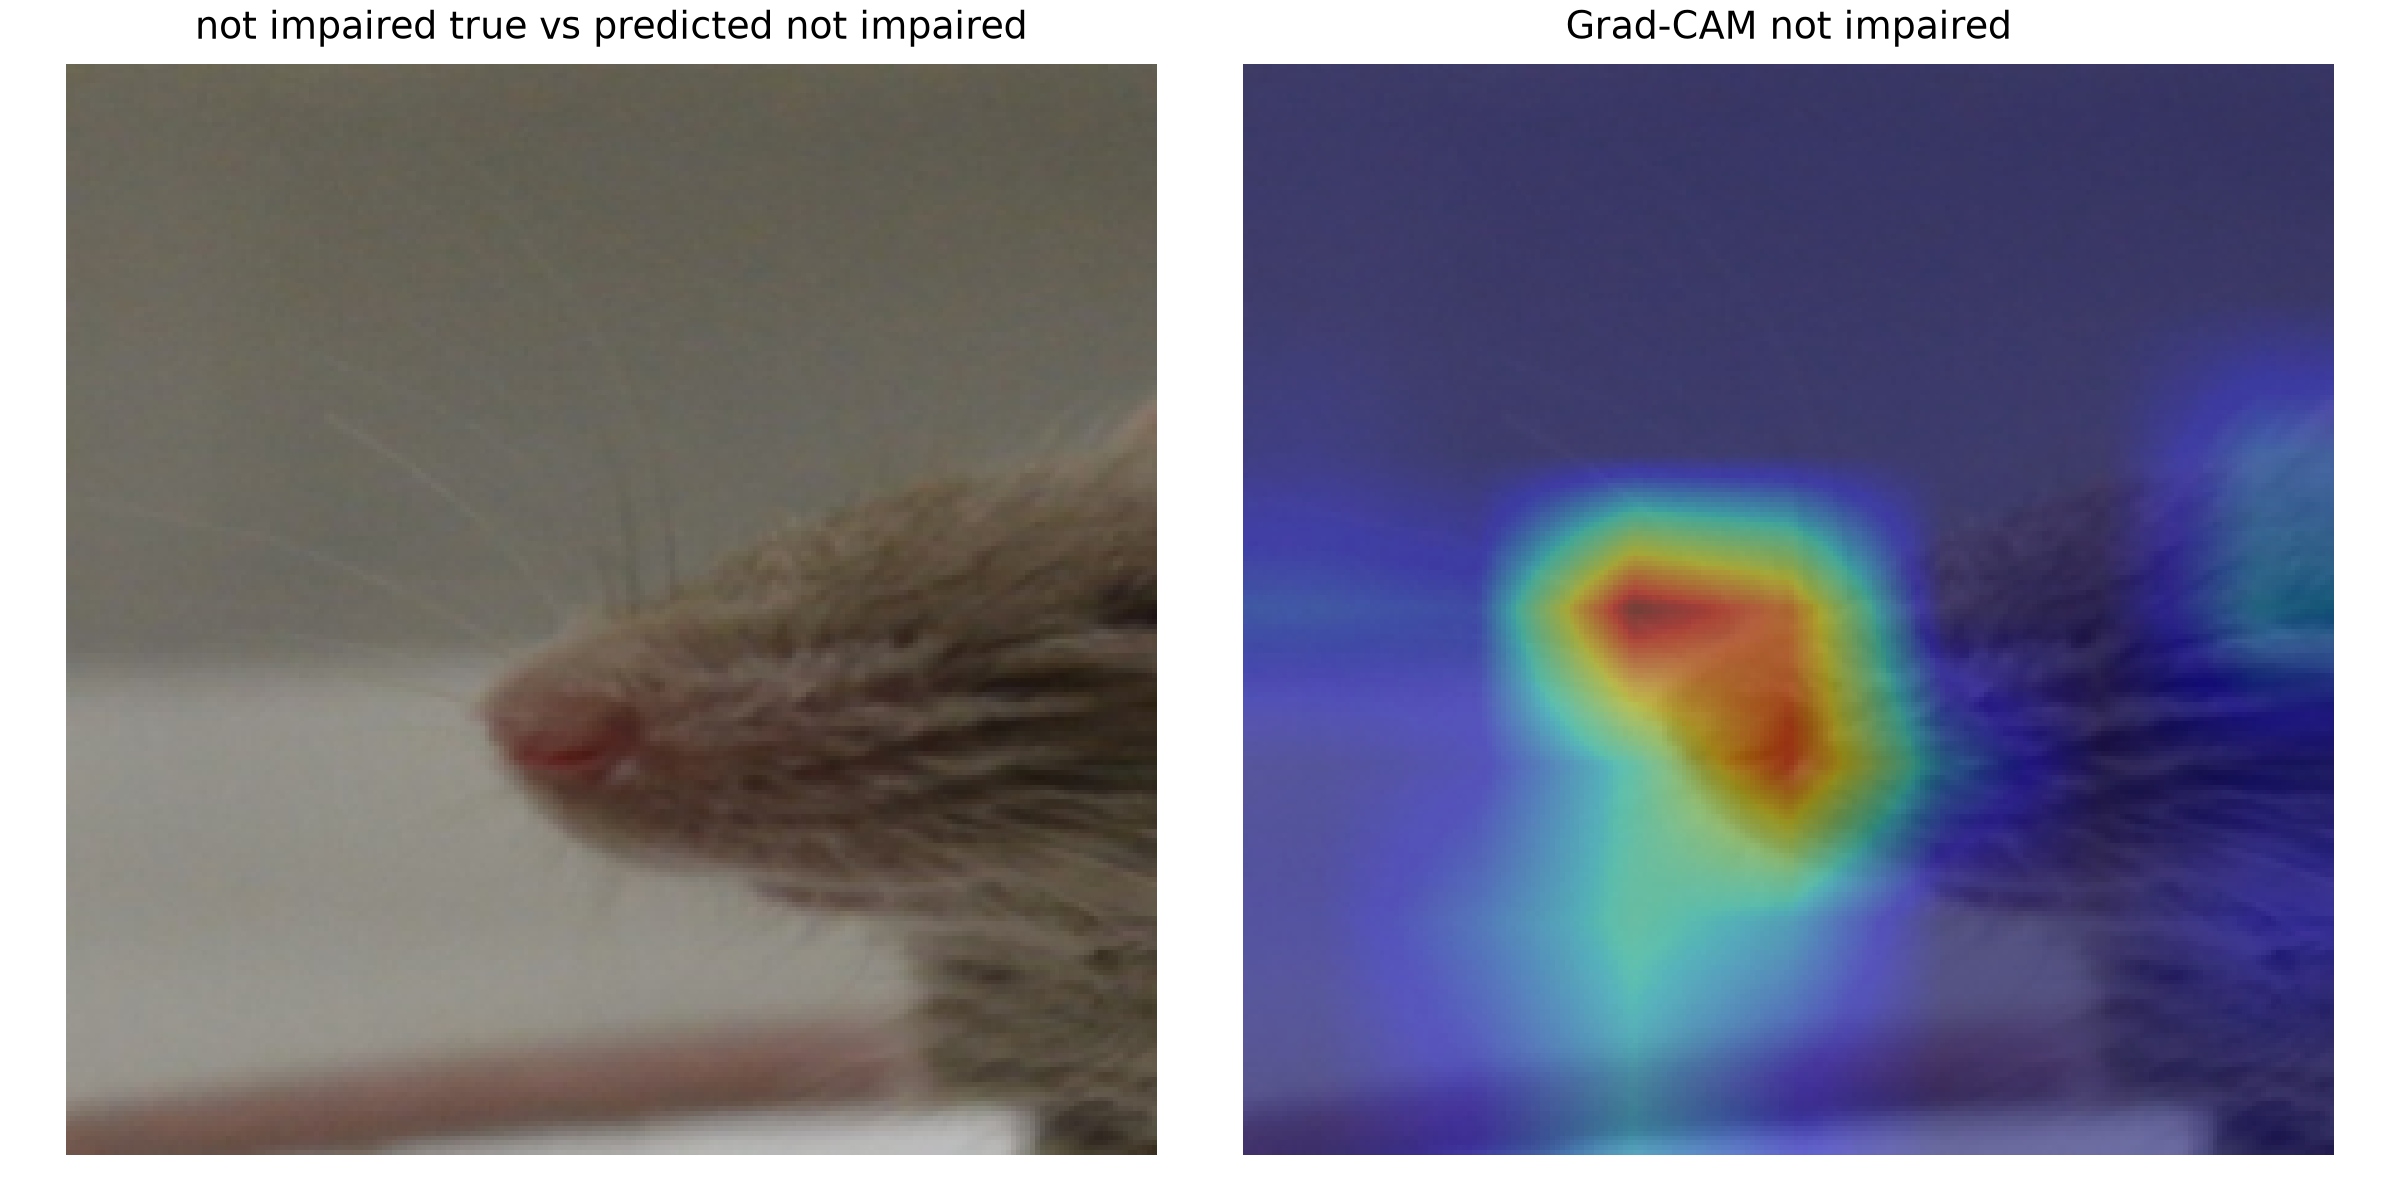
\includegraphics[width=\linewidth]{figures/qualitative/crop_tn_gradcam.png}
    \caption{Crop, correct not-impaired (Grad-CAM).}
    \label{fig:q-crop-tn-gc}
  \end{subfigure}\hfill
  \begin{subfigure}[t]{0.32\textwidth}
    \centering
    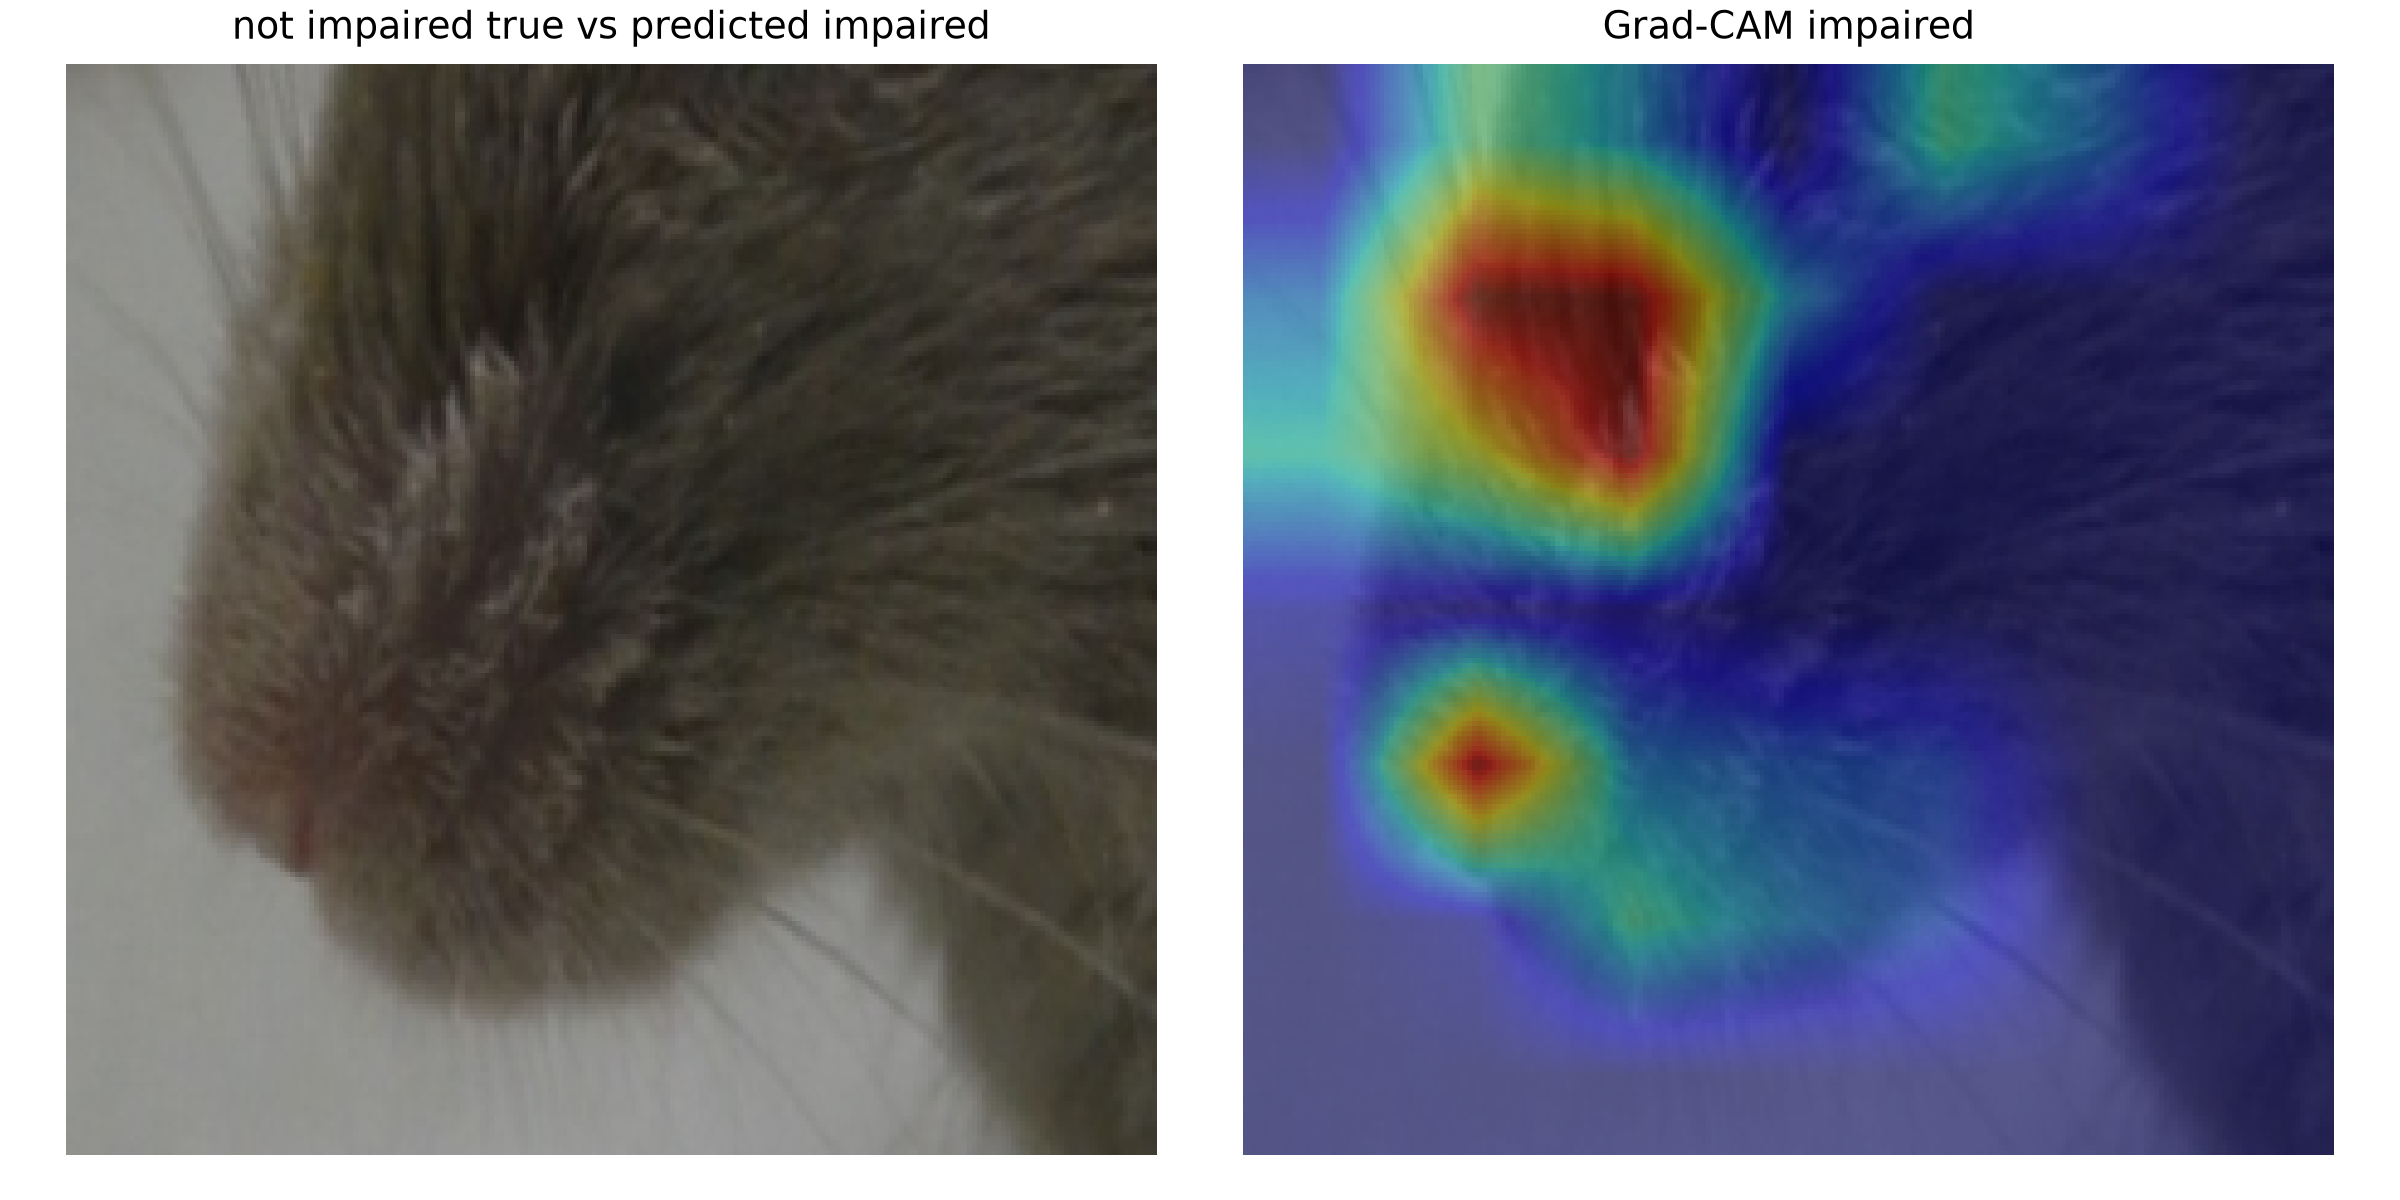
\includegraphics[width=\linewidth]{figures/qualitative/crop_fp_gradcam.png}
    \caption{Crop, false impaired (Grad-CAM).}
    \label{fig:q-crop-fp}
  \end{subfigure}

  \vspace{0.45em}

  \begin{subfigure}[t]{0.32\textwidth}
    \centering
    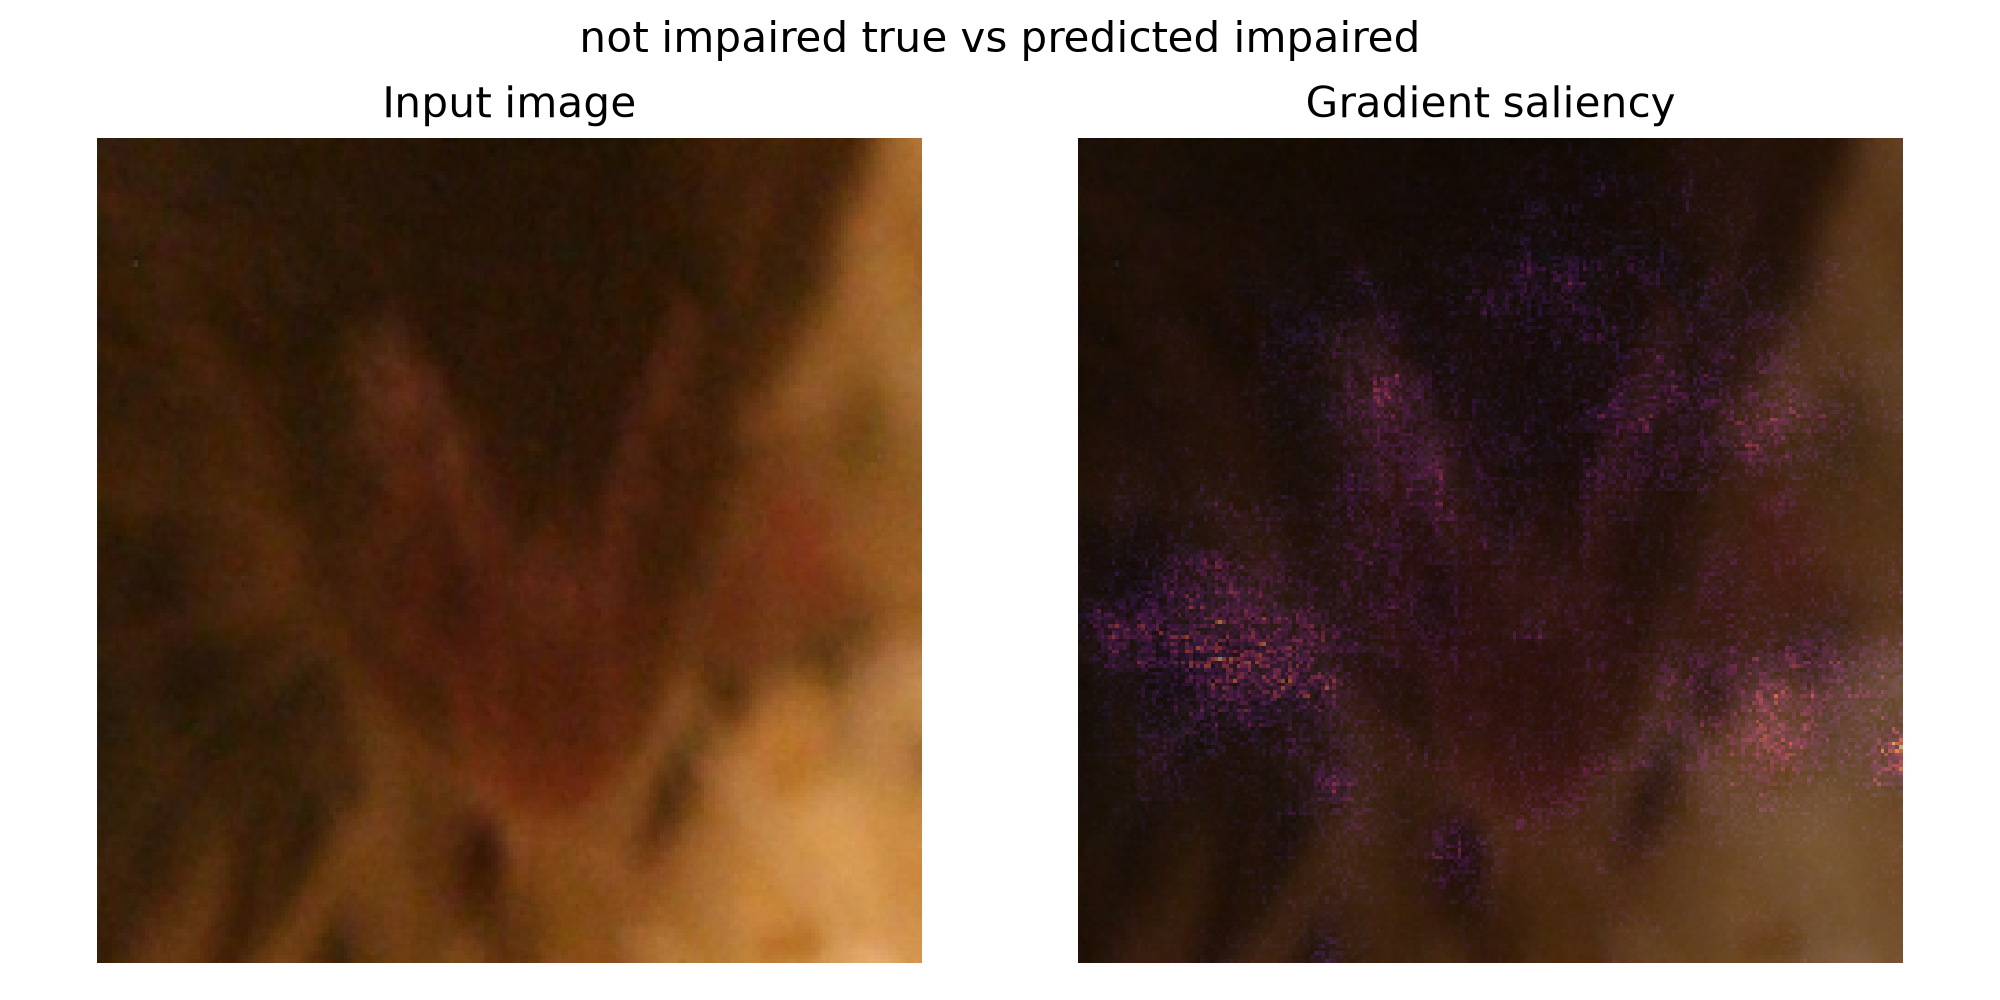
\includegraphics[width=\linewidth]{figures/qualitative/crop_fp_saliency.png}
    \caption{Crop, false impaired (saliency).}
    \label{fig:q-crop-fp-sal}
  \end{subfigure}\hfill
  \begin{subfigure}[t]{0.32\textwidth}
    \centering
    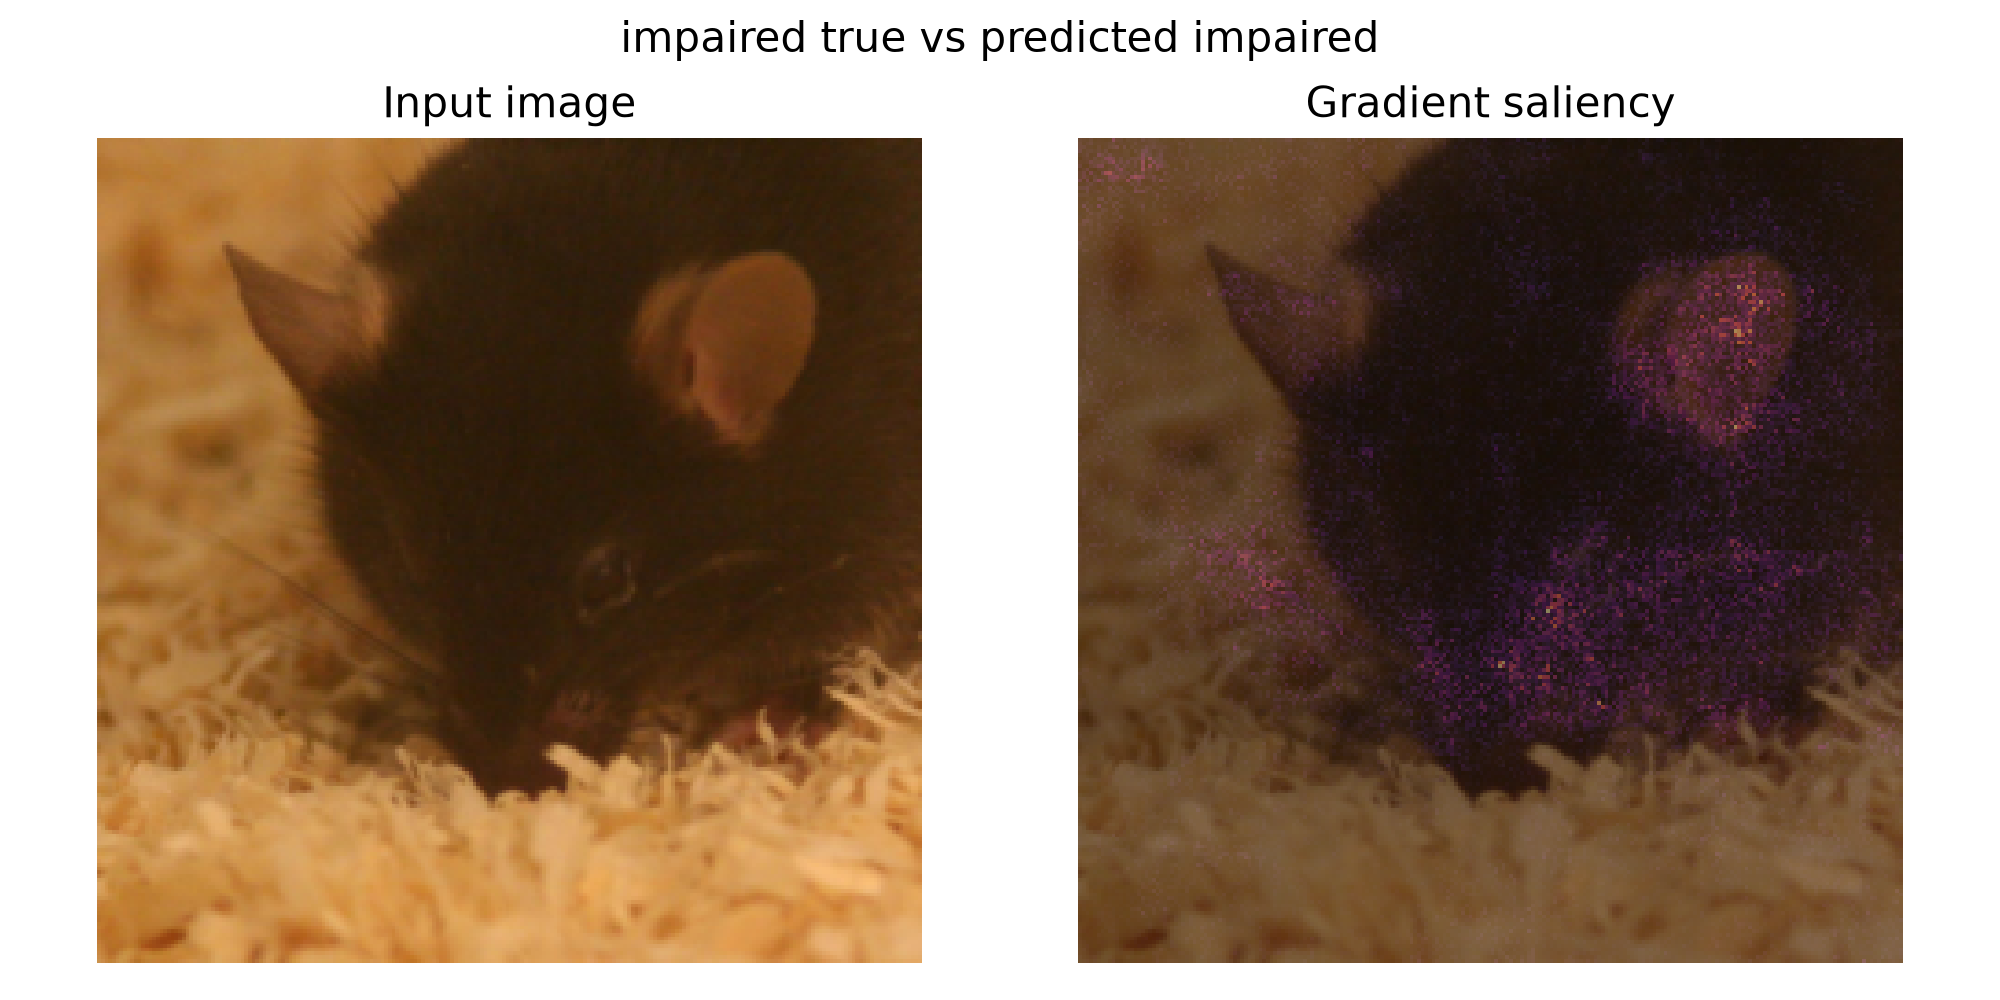
\includegraphics[width=\linewidth]{figures/qualitative/full_tp_saliency.png}
    \caption{Full, correct impaired (saliency).}
    \label{fig:q-full-tp}
  \end{subfigure}\hfill
  \begin{subfigure}[t]{0.32\textwidth}
    \centering
    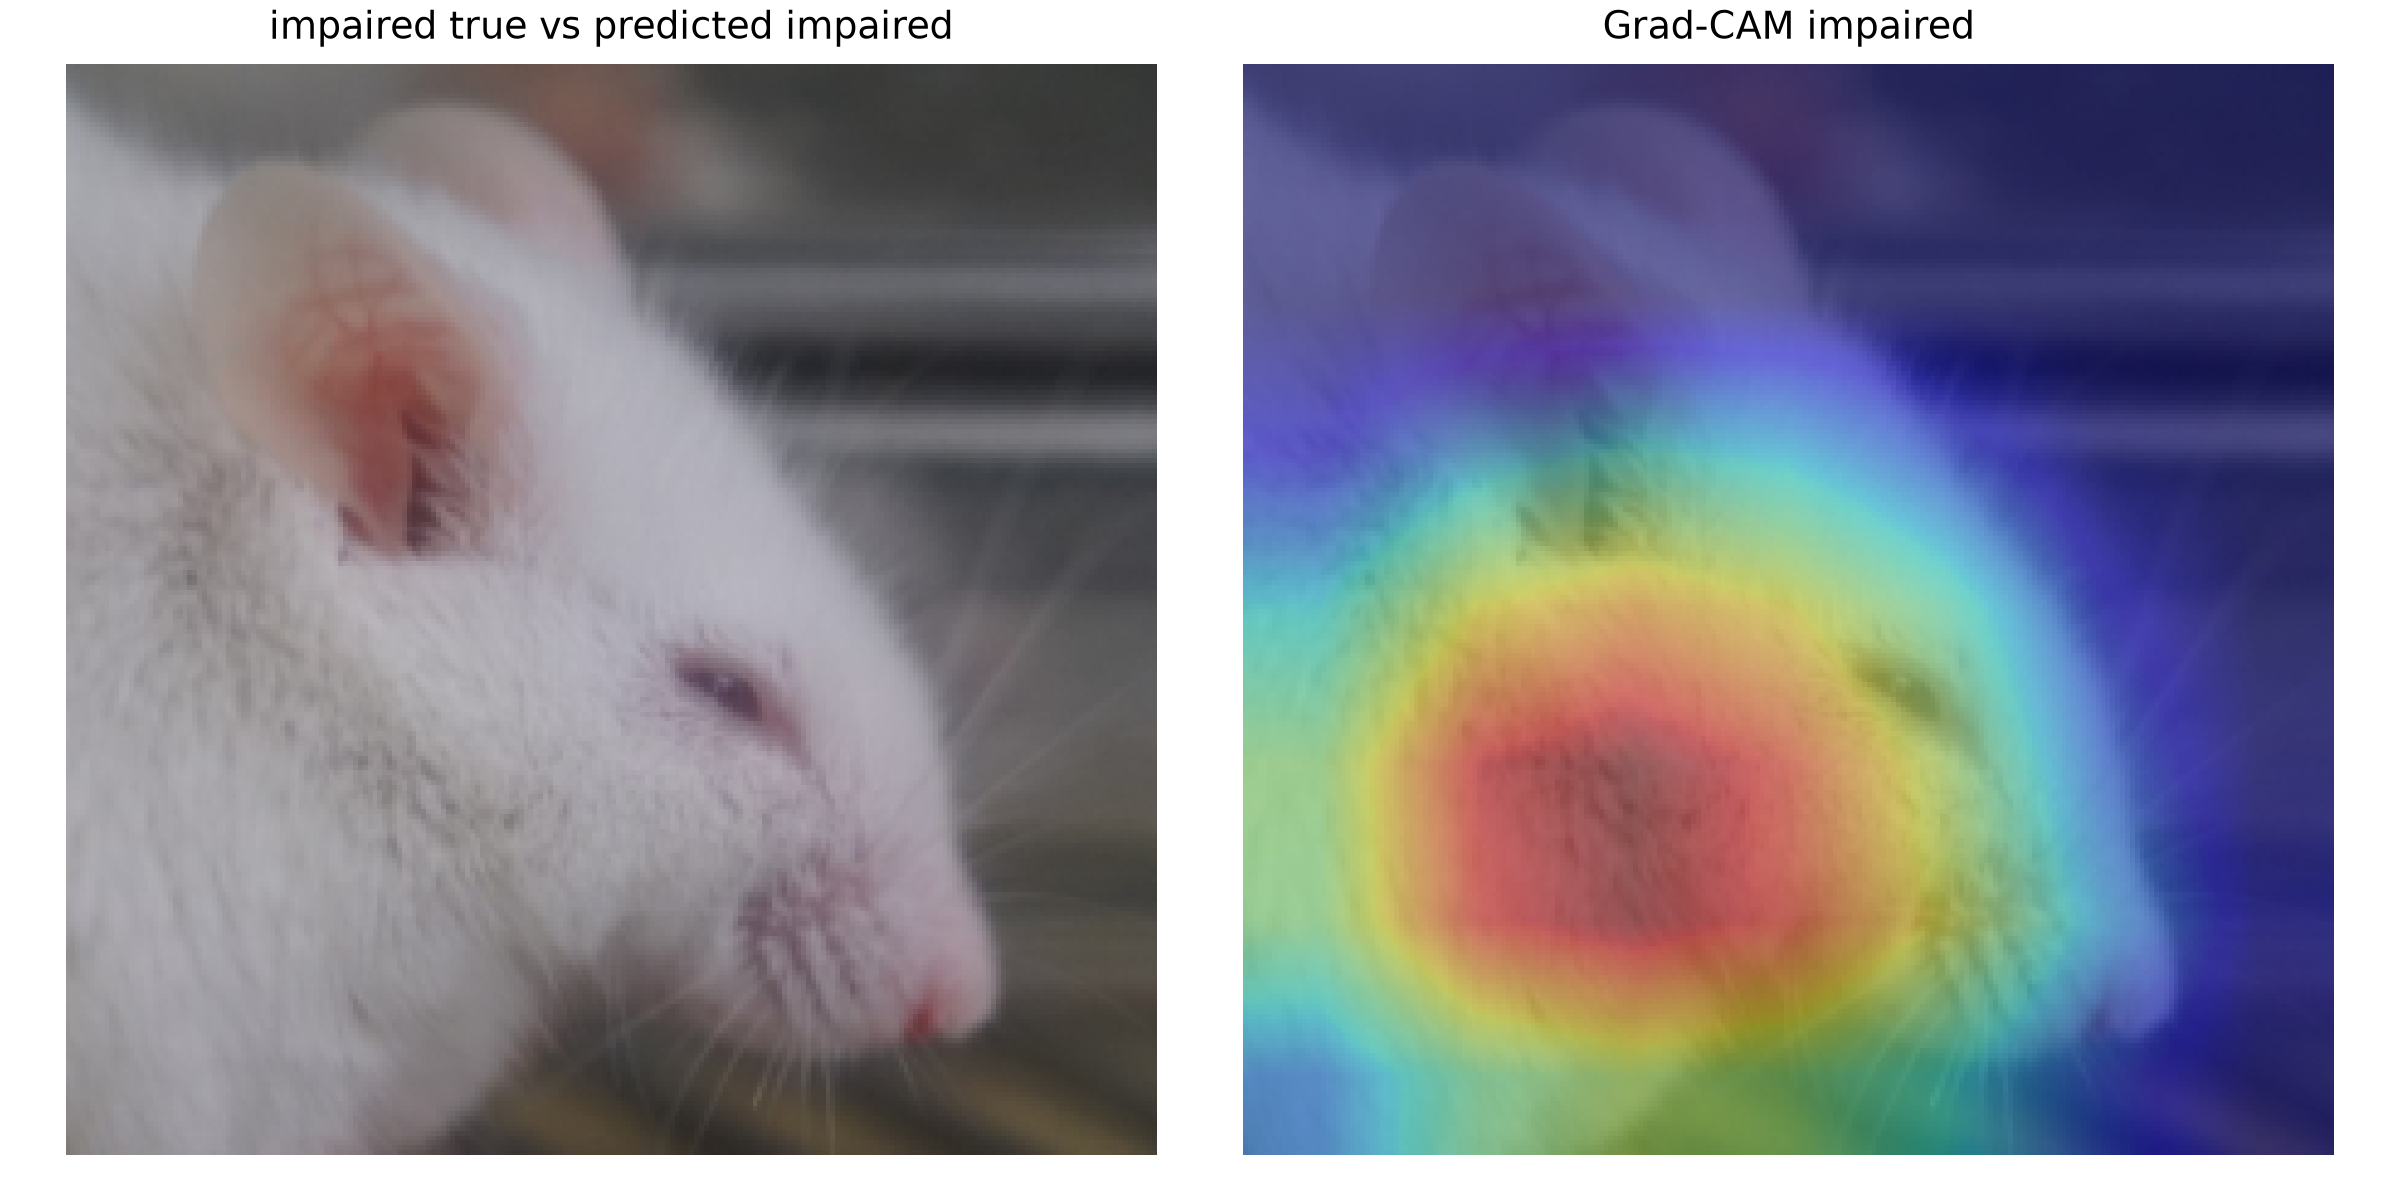
\includegraphics[width=\linewidth]{figures/qualitative/full_tp_gradcam.png}
    \caption{Full, correct impaired (Grad-CAM).}
    \label{fig:q-full-tp-gc}
  \end{subfigure}

  \vspace{0.45em}

  \begin{subfigure}[t]{0.32\textwidth}
    \centering
    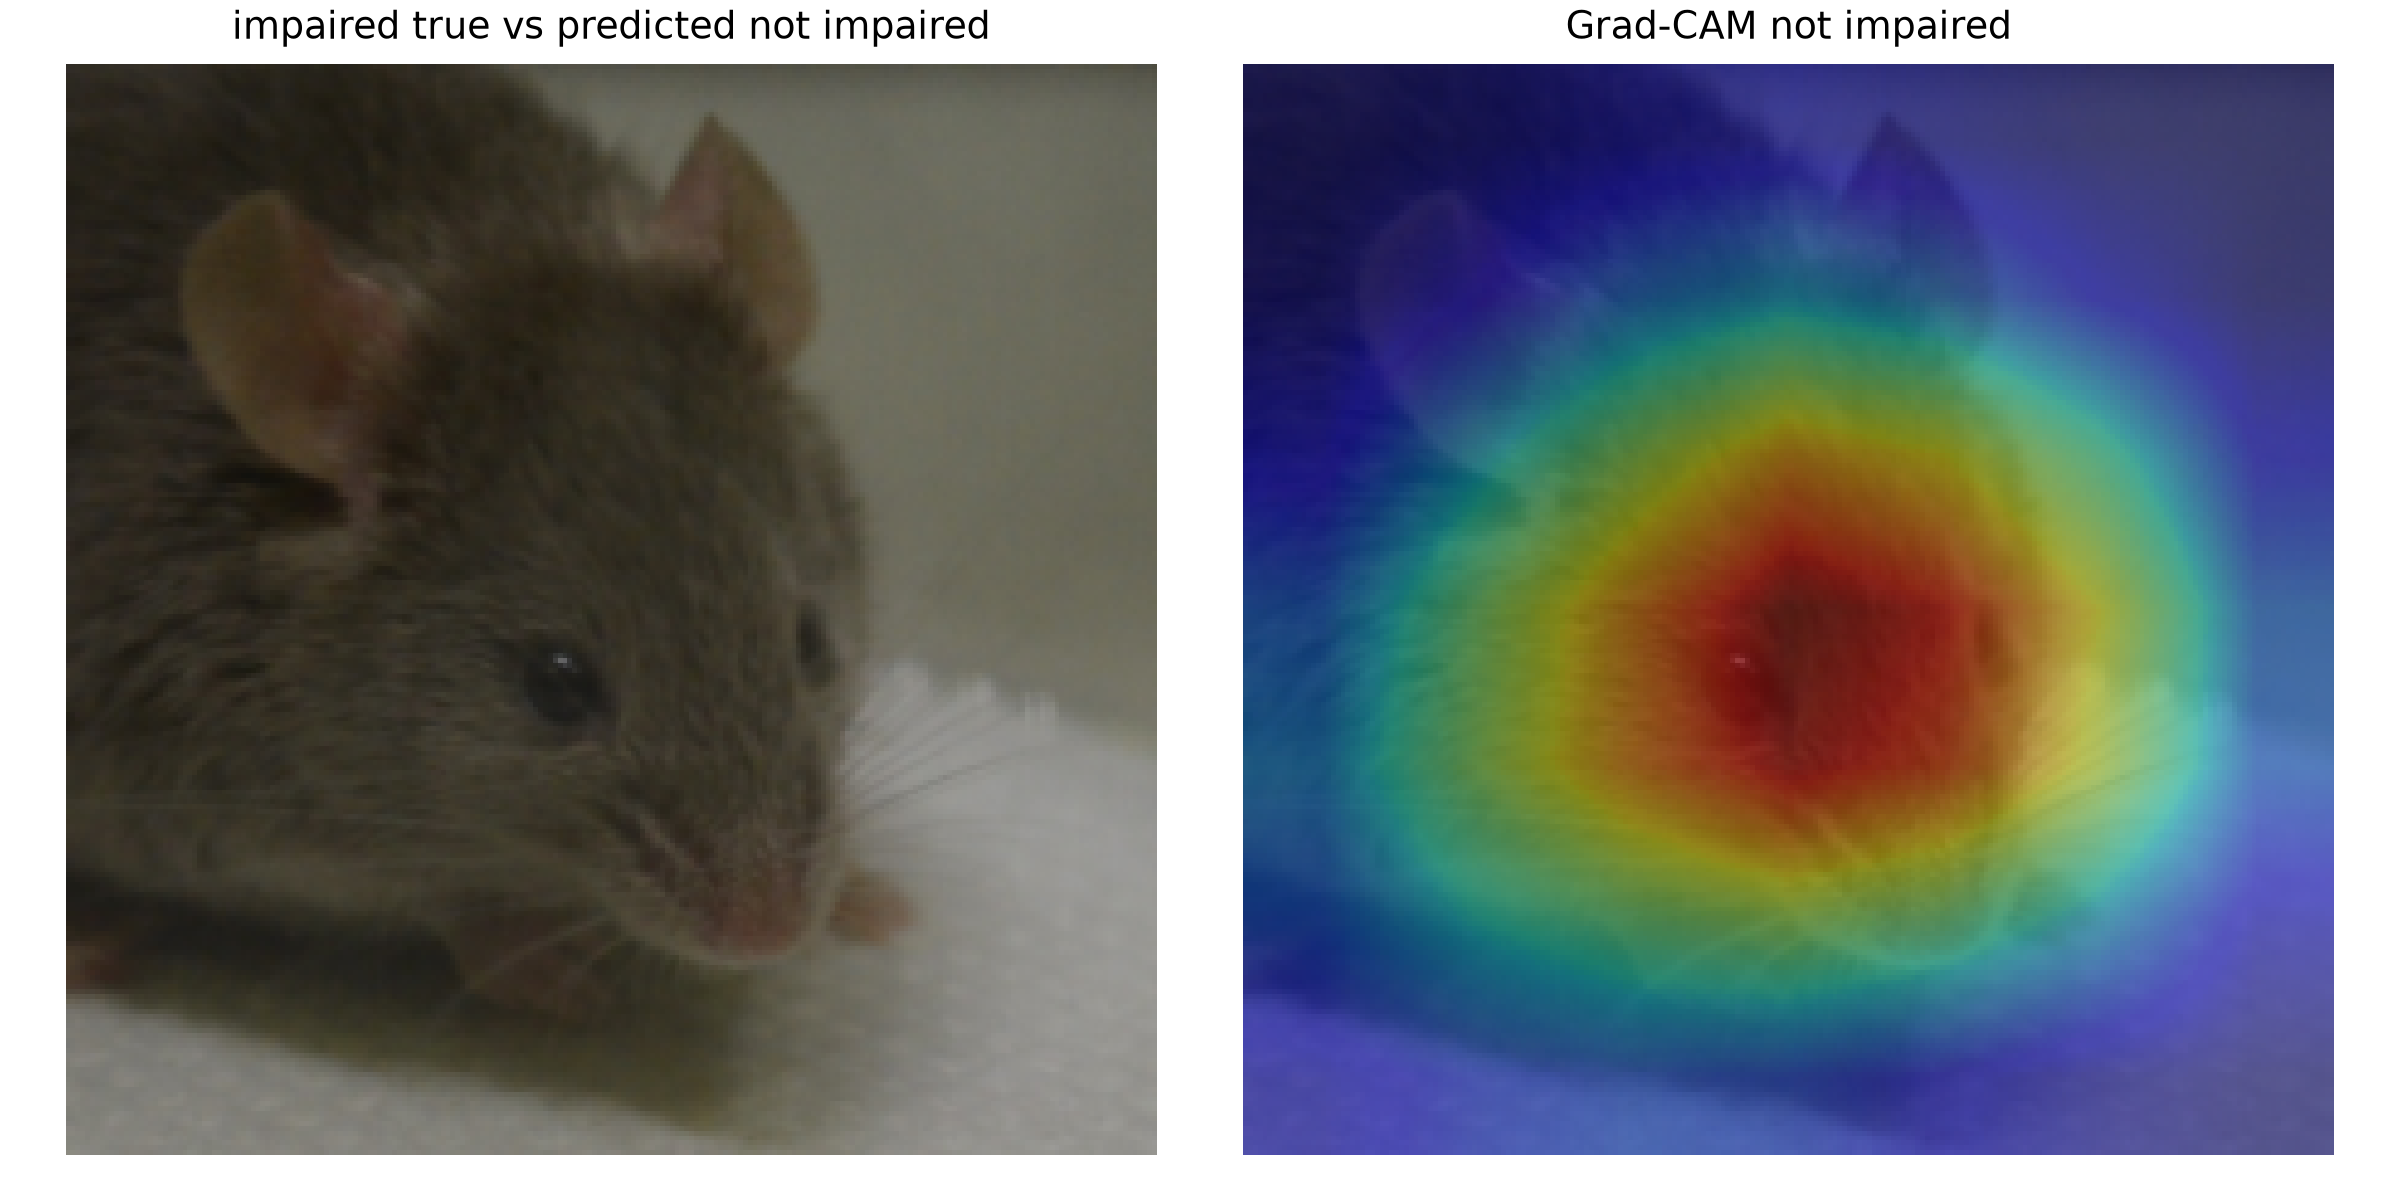
\includegraphics[width=\linewidth]{figures/qualitative/full_fn_gradcam.png}
    \caption{Full, missed impaired (Grad-CAM).}
    \label{fig:q-full-fn}
  \end{subfigure}\hspace{0.02\textwidth}
  \begin{subfigure}[t]{0.32\textwidth}
    \centering
    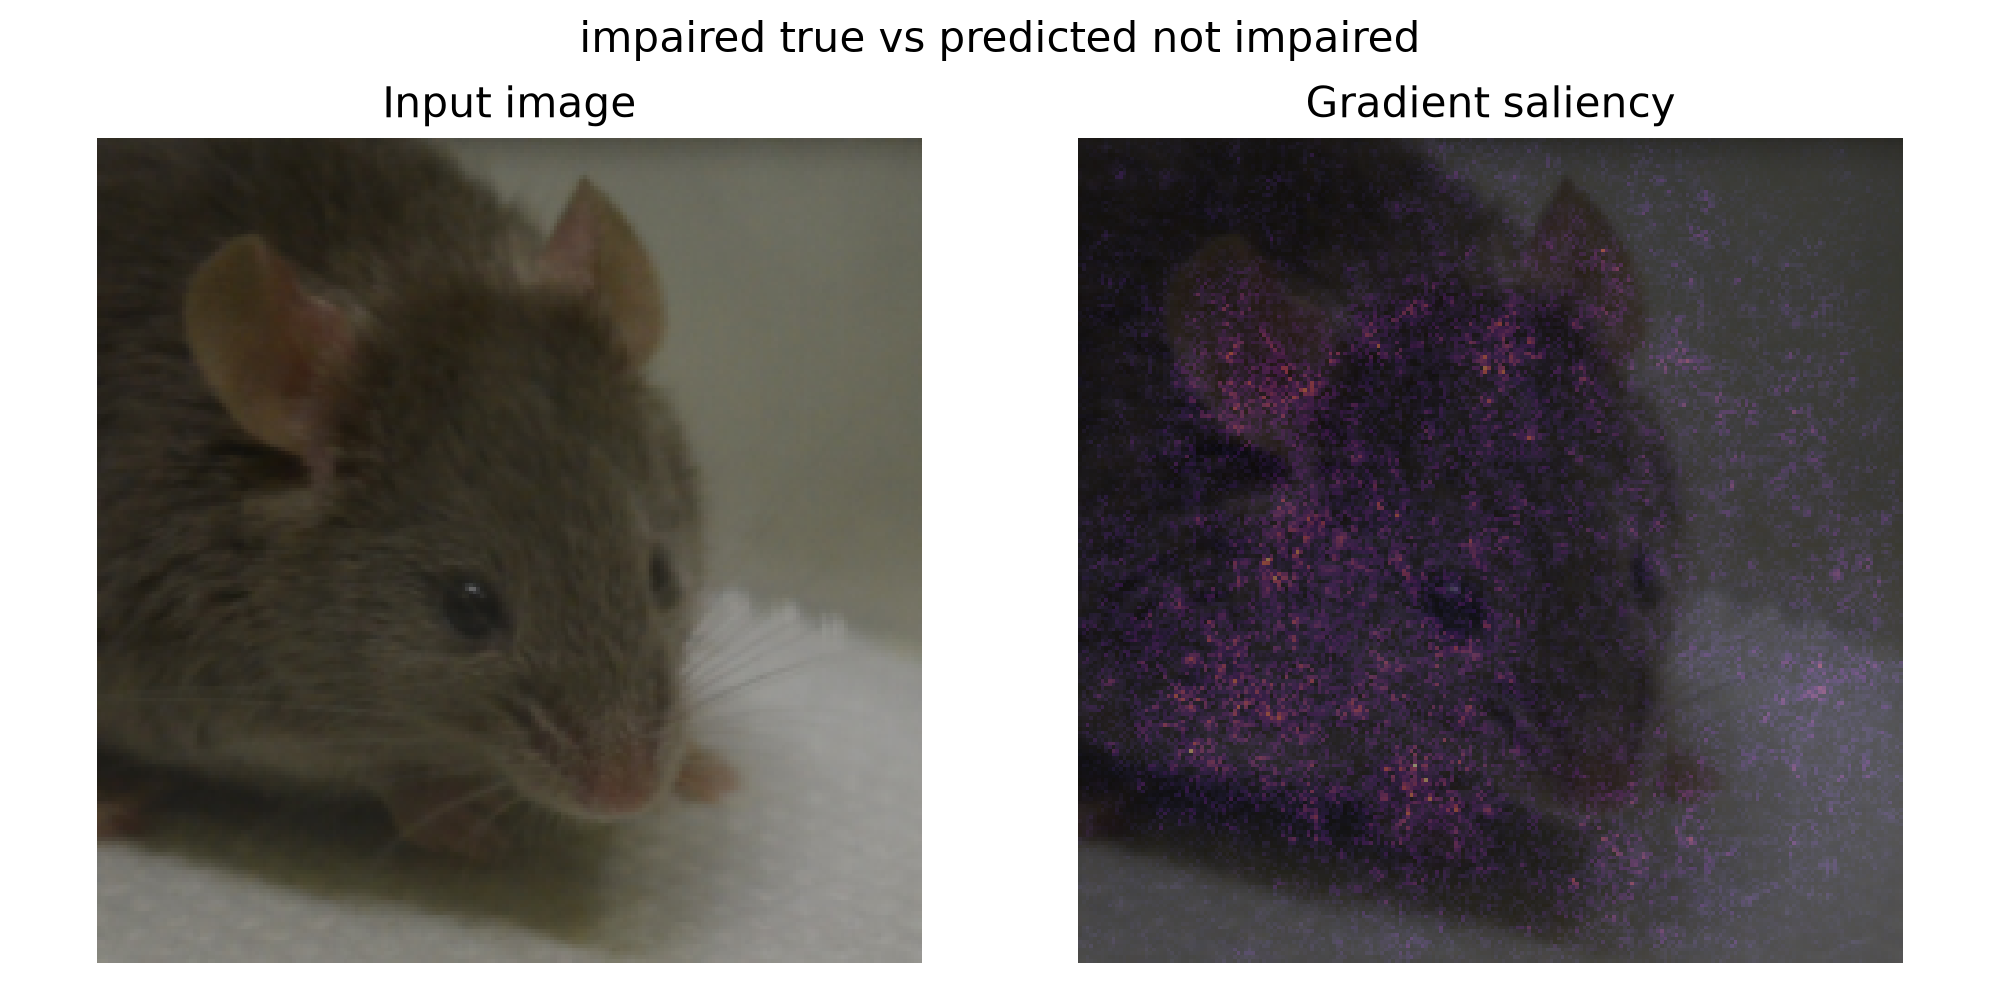
\includegraphics[width=\linewidth]{figures/qualitative/full_fn_saliency.png}
    \caption{Full, missed impaired (saliency).}
    \label{fig:q-full-fn-sal}
  \end{subfigure}
  \caption{Selected qualitative examples from the best crop and full-image
  models. Left: input; right: Grad-CAM or gradient saliency for the predicted
  class.}
  \label{fig:qualitative}
\end{figure*}

%% ================================================================
%%  DISCUSSION
%% ================================================================
\section{Discussion}
\label{sec:discussion}

\paragraph{Muzzle crops are informative, but full images remain strongest
overall.}
The best crop model achieves Macro-F1~$=0.812$, closing to within $2.6$~pp of
the best full-image result ($0.838$). This supports the hypothesis that
well-being status leaves detectable traces in the muzzle region alone. From
a practical standpoint, muzzle-only pipelines are attractive because they
require smaller sensors or tighter camera framing and avoid capturing
background features that could act as confounds. However, the consistent
advantage of full-image inputs---driven primarily by ResNet18's large
crop-to-full gap ($+7.1$~pp in Part~1)---indicates that peripheral facial cues
(orbital tightening, ear position, cheek shape) carry complementary
information. Per-class analysis reinforces this: the full-image model's
specificity ($0.881$) and sensitivity ($0.780$) both exceed the crop model's
($0.821$ and $0.742$), suggesting that full frames offer better
discrimination for both classes.

\paragraph{Light augmentation and fine-tuning matter, but the gains are
architecture-dependent.}
ResNet18 benefits dramatically from light augmentation: Macro-F1 on full
images increases by $5.7$~pp, the single largest improvement observed in the
entire study. This is consistent with ResNet18's smaller parameter count
($11.7$M), which makes it more susceptible to overfitting on a dataset of
${\sim}1{,}250$ training images. In contrast, ConvNeXt-Tiny ($28.6$M
parameters) shows minimal augmentation sensitivity, gaining only $0.8$~pp on
crops and losing $0.1$~pp on full images. We hypothesize that ConvNeXt-Tiny's
built-in stochastic depth and layer-scale regularization partially substitute
for external augmentation. In Part~2, reducing the learning rate from
$10^{-4}$ to $5\times10^{-5}$ provides a further $0.8$~pp gain for ResNet18,
while raising it to $3\times10^{-4}$ hurts ConvNeXt ($-2.6$~pp),
underscoring the sensitivity of pretrained feature adaptation to update
magnitude.

\paragraph{Architecture interacts with input type.}
ConvNeXt-Tiny is the stronger crop model in Part~1 ($0.797$ vs.\ $0.759$ for
ResNet18 with augmentation) and closes the crop--full gap nearly completely.
After Part~2 tuning, ConvNeXt crop reaches $0.812$, compared to $0.838$ for
ResNet18 full. The interaction is architecturally interpretable: ConvNeXt's
$7\times7$ depthwise convolutions cover a larger fraction of the $224\times224$
muzzle crop than ResNet18's $3\times3$ kernels, enabling it to capture
coarser shape deformations (e.g., nose bulge) in fewer layers. On full images,
the additional spatial context benefits ResNet18's hierarchical aggregation.
This suggests that model choice should be conditioned on the intended
acquisition setup---a tightly framed muzzle camera favors ConvNeXt-Tiny,
whereas a broader face view favors ResNet18.

\paragraph{Full fine-tuning is essential.}
Freezing the ConvNeXt backbone and training only the classification head
reduces Macro-F1 by $1.9$~pp, confirming that ImageNet features do not fully
transfer to the mouse facial domain. This is expected: ImageNet contains no
rodent faces, and the low-level textures (fur, whiskers, skin tones) differ
substantially from natural photographic scenes. The frozen-backbone
ROC-AUC ($0.849$) remains competitive, suggesting that ImageNet features
partially capture useful structure, but the gain from end-to-end fine-tuning
is consistent and significant.

\paragraph{Prediction confidence and threshold robustness.}
The bimodal prediction probability distributions (Figure~\ref{fig:prob-hist})
indicate that both models produce confident outputs for the majority of test
samples. Threshold sensitivity analysis (Figure~\ref{fig:threshold-curves})
confirms that Macro-F1 varies by less than $3$~pp across thresholds from $0.2$
to $0.7$, demonstrating that the reported results are not artifacts of a
particular threshold choice. This stability is encouraging for deployment,
where the operating threshold may need adjustment to balance sensitivity and
specificity for specific welfare protocols.

\paragraph{Subset variation reveals domain-shift challenges.}
The per-subset analysis (Table~\ref{tab:subset}) exposes substantial
performance heterogeneity. KH and JW, which together contribute the largest
training populations, achieve Macro-F1 above $0.87$. MR, despite being the
largest single subset, underperforms ($0.744$), possibly due to differences in
camera setup, lighting, or mouse strain. AW achieves only $0.575$, but its
test set contains merely $13$ images ($5$ impaired), making this estimate
unreliable. The LW subset shows high raw accuracy ($0.941$) but severe class
imbalance ($29$ not-impaired vs.\ $5$ impaired), yielding a lower balanced
accuracy ($0.800$). These findings highlight that cross-subset generalization
remains a challenge, and that stratified evaluation by recording condition is
essential for realistic performance assessment.

\paragraph{Limitations.}
Several factors constrain the generality of our findings. First, the curated
dataset ($1{,}778$ images) represents a small fraction of the original
${\sim}35{,}000$ image pool; many images lacked MGS annotations or had
incomplete ratings. Second, muzzle crops were prepared with substantial manual
effort, which limits scalability. Third, binary labels derived from a
mean-score threshold of $0.5$ collapse the ordinal MGS scale into a coarse
dichotomy; alternative thresholds or multi-class formulations may capture
finer welfare gradations. Fourth, inter-rater variability in the original
MGS annotations introduces label noise whose impact on model training and
evaluation we do not quantify. Fifth, the five subsets span different labs,
experimenters, and possibly mouse strains, but our study does not include an
explicit cross-lab validation protocol. Finally, all experiments use a single
train/val/test split; cross-validation would provide more robust estimates
at the cost of increased computation.

\paragraph{Future work.}
Several directions could address the limitations above and extend the
practical impact of this work. (i)~\emph{Automated muzzle localization}: using
DeepLabCut keypoints or a lightweight detection network to replace manual
cropping would enable end-to-end pipelines from raw video. (ii)~\emph{Threshold
optimization}: selecting the decision threshold on the validation set (e.g.,
via Youden's J statistic) could improve sensitivity for the impaired class
without substantial loss in specificity. (iii)~\emph{Expanded labeled data}:
increasing the annotated pool and adding multi-class labels (e.g., mild vs.\
moderate vs.\ severe impairment) would test model resolution beyond binary
classification. (iv)~\emph{Cross-lab validation}: evaluating models trained on
one subset and tested on another would quantify domain-shift robustness.
(v)~\emph{Temporal modeling}: incorporating video sequences rather than single
frames could exploit temporal dynamics of facial expressions for more reliable
welfare assessment.

%% ================================================================
%%  CONCLUSION
%% ================================================================
\section{Conclusion}
\label{sec:conclusion}

We presented a reproducible deep-learning study of binary mouse well-being
classification from images. Using MGS-derived labels and a fixed
subset/class-stratified split, we compared ResNet18 and ConvNeXt-Tiny on muzzle
crops and full images across $14$ experimental configurations. The best overall
system is full-image ResNet18 with light augmentation and learning rate
$5\times10^{-5}$ (Macro-F1 $=0.838$, specificity $=0.881$, sensitivity
$=0.780$). The best crop-only system is ConvNeXt-Tiny with light augmentation
and dropout $0.0$ (Macro-F1 $=0.812$). Light augmentation substantially
improves ResNet18 ($+5.7$~pp), while full fine-tuning consistently outperforms
frozen backbones ($+1.9$~pp). Prediction confidence is high and threshold
sensitivity is low, supporting deployment with a default threshold. Per-subset
analysis reveals domain-shift challenges that motivate future cross-lab
validation. Together, these findings support automatic, non-invasive well-being
assessment from mouse muzzle imagery and provide a clear experimental baseline
for future extensions.

\begin{acks}
This work was carried out as part of the Hot Topics in Computer Vision project
at TU Berlin (2026).
\end{acks}

\bibliographystyle{ACM-Reference-Format}
\bibliography{references}

\end{document}
